% LTex: language=pl
\documentclass{szablonPG}
\usepackage[style=numeric, language=polish, backend=bibtex, sorting=none]{biblatex}
\usepackage{dirtree}
\usepackage{listing_schemat}
\DeclareDelimFormat{finalnamedelim}{\addspace i\space}

% Żródła bibliografii
\addbibresource{bibliography/intro.bib}
\addbibresource{bibliography/elastic.bib}
\addbibresource{bibliography/bibliography.bib}
\addbibresource{bibliography/k8s.bib}
\addbibresource{bibliography/docker.bib}
\addbibresource{bibliography/hardware.bib}
\addbibresource{bibliography/analiza.bib}
\addbibresource{bibliography/xcp.bib}
\addbibresource{bibliography/python.bib}
\addbibresource{bibliography/linux.bib}
\addbibresource{bibliography/windows.bib}
\addbibresource{bibliography/wine.bib}
\addbibresource{bibliography/nix.bib}
\addbibresource{bibliography/misc.bib}
\addbibresource{bibliography/sqlite.bib}
% Koniec zrodel
\begin{document}
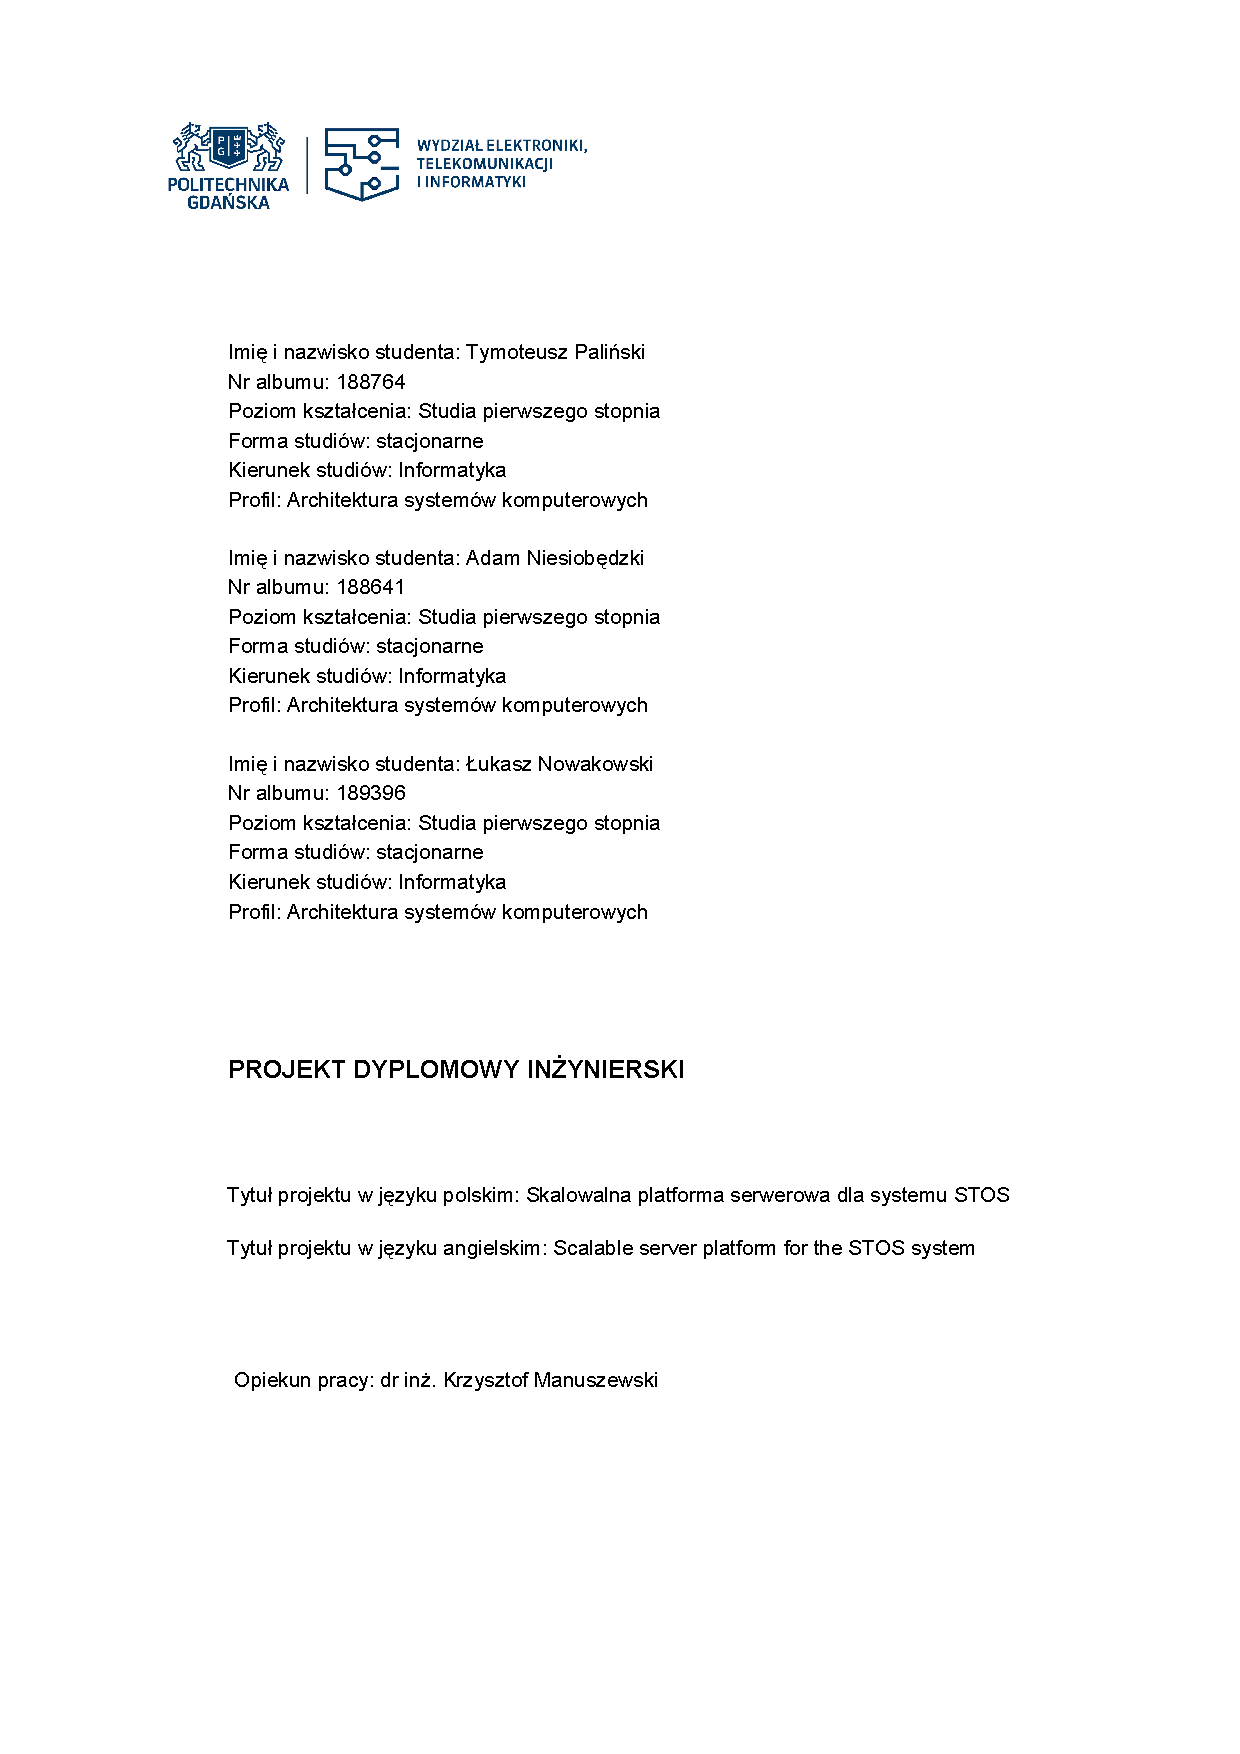
\includepdf{meta/StronaTytulowa.pdf}

% druga strona musi być pusta i nienumerowana
\newpage
\thispagestyle{empty}
\mbox{}
\newpage

% Rzeczy typu nagłówek, etc.
% LTex: language=pl
\chapter*{Streszczenie}
\indent Lorem Lorem ipsum dolor sit amet, consectetur adipiscing elit. Vivamus elementum arcu nec blandit aliquam. Integer eros dolor, molestie eget dictum quis, luctus sit amet sapien. Proin dignissim felis in ornare volutpat. Morbi vulputate rutrum efficitur. Ut vehicula vehicula metus, et iaculis tortor mattis vel. Nam blandit, arcu quis ultricies blandit, libero ante commodo augue, in accumsan dui leo at orci. Phasellus in augue et velit pulvinar malesuada ut et sem. Nulla vehicula nibh eu odio sollicitudin sagittis. Praesent condimentum semper neque, tincidunt luctus nisl scelerisque sed. Orci varius natoque penatibus et magnis dis parturient montes, nascetur ridiculus mus. 
\vspace{0.5cm}\newline
\textbf{Słowa kluczowe:} lorem ipsum, dolor sit amet, consectetur adipiscing\vspace{0.5cm}

\noindent \textbf{Dziedzina nauki i techniki, zgodnie z wymogami OECD:} nauki inżynieryjne i techniczne, robotyka i automatyka

\chapter*{Abstract}
\indent STOS, or Student Testing and Grading System \textit{(System testowania i oceny studentów)} is a system used extensively as a part of the educational process at Faculty of Electronics, Telecommunications and Informatics at Gdańsk Tech. It acts as the backbone of the procedure of automatic grading of practical assignments submitted by students, which helps the course instructors with timely evaluation of the students' work.
\newline \noindent In this paper, we explore the process of analysis of the documentation and source code of the existing system, evolution of the concepts regarding the creation of a solution and finally, the implementation of a scalable server platform for the STOS system. A number of enterprise grade technologies and their use in context of the existing system is presented, in order to paint a clear picture of the choices made in relation to the implementation of the server platform. Both the solution implemented using Python in form of a backend application and configuration of a multi node server environment for said application are explored, embedding the theoretical analysis of used technologies in a more practical context. Finally, a brief summary of the solution is given, including possible future improvements to the server platform of the STOS system.
\vspace{0.5cm}\newline
\textbf{Keywords:} scalable server platform, distributed systems, cloud computing, containerization, virtualization \vspace{0.5cm}

\tableofcontents

% Rozdziały
% LTex: language=pl
\chapter{Wstęp (autor: Łukasz Nowakowski)}

% LTex: language=pl
\section{Opis systemu STOS}
\indent System Testowania i~Oceny zadań Studenckich (w skrócie „STOS”), to system dedykowany dla prowadzących zajęcia na Politechnice Gdańskiej. Umożliwia testowanie rozwiązań stworzonych przez studentów podczas zajęć projektowych oraz laboratoryjnych, pod kątem wydajności i~poprawności. Przepływ pracy polega na przesłaniu kodu programu przez studenta do systemu, kompilacji po stronie serwera oraz przesłaniu wyniku na podstawie serii testów zdefiniowanych przez prowadzącego.

\section{Komponenty i~schemat działania}
System możemy podzielić na komponenty ze względu na realizowane zadania:
\begin{itemize}
    \item STOS -- serwis w~postaci strony internetowej, umożliwiający wgranie rozwiązań przez studentów i~umieszczenie ich w~kolejce dostępnej do pobrania przez inne serwisy poprzez żądania HTTP.
    \item Moduł sprawdzający -- część serwisu działającego po stronie serwera. Jego zadaniem, jest wywoływanie zapytań do API STOS-u metodą odpytywania, w~celu pobierania kodu programów do wykonania, zlecenie kompilacji, ocenę kodu oraz przesłanie wyniku do STOS-u.
    \item Moduł kompilujący -- skonteneryzowany serwis działający na serwerze, kompilujący otrzymany kod. Ma możliwość kompilacji lub interpretacji wielu języków programowania. Aktywnie nasłuchuje komunikatów przesyłanych przez nazwany potok. Jest przystosowany do ciągłego działania, co wymaga uruchomienia go wyłącznie przy starcie całej platformy. Posiada współdzielone katalogi z~gospodarzem, zawierające skrypty kontrolujące, kody źródłowe oraz rezultaty.
\end{itemize}
\begin{figure}
	\begin{center}
		\resizebox{1.0\textwidth}{!} {
			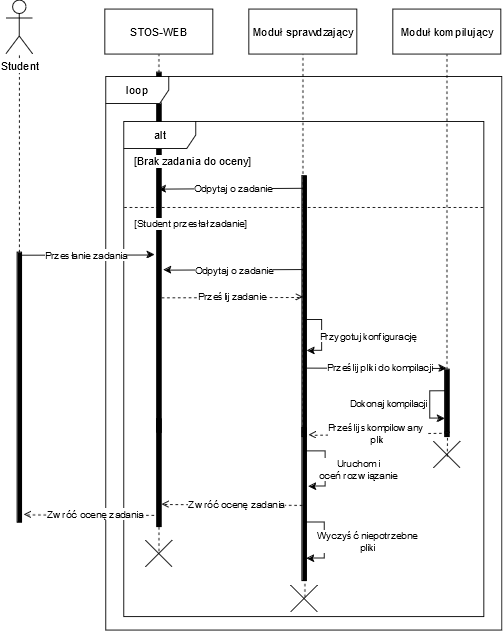
\includegraphics{img/1/d_sek_1.png}
		}
		\caption[Diagram sekwencji komponentów]{Diagram przedstawiający sekwencję wykonywanych zdarzeń w~systemie, podczas oceny zadania. Źródło własne.}
	\end{center}
\end{figure}


% LTex: language=pl
\section{Problemy aktualnego systemu i~propozycja rozwiązań}
\indent Obecnie, system używa pojedynczych instancji każdego z~komponentów. Skutkiem jest zwiększenie przewidywalności działania oraz uproszczenie struktury kodu. Badając czas działania komponentów, można zauważyć, że moduł kompilujący wykonuje się najdłużej. Jest to spodziewany rezultat, ze względu na konieczność skanowania, analizowania, optymalizowania i~generowania kodu \cite{procesKompilacji}. Ten proces jest powtarzany dla każdego zadania, co już przy niewielkiej liczbie studentów publikujących kod w~tym samym czasie, powoduje znaczne wydłużenie czasu oczekiwania na wynik. Szczególnie widoczne jest to w~okresie końcowych terminów przesyłania zadań projektowych, które często zawierają skomplikowaną do kompilacji i~oceny logikę. Skutecznym i~prostym rozwiązaniem byłoby uruchomienie kilku instancji modułu kompilującego pracujących jednocześnie. Moduł ten jest przystosowany do uruchamiania w~postaci kontenera działającego na platformie do konteneryzacji Docker, co ułatwia proces tworzenia nowych instancji. Przeszkodą jest konieczność synchronizacji między modułem sprawdzającym a~wieloma modułami kompilującymi. Ich komunikacja odbywa się poprzez przesyłanie tekstowych wiadomości przez nazwany potok. Przy nasłuchującym trybie pracy wszystkich modułów kompilujących, będą one konkurować o~odczyt danych. Skutkiem jest niepoprawne pobranie komendy z~potoku. Z~racji okresowego występowania zwiększenia zapotrzebowania na moc obliczeniową systemu, nie jest wymagane, by uruchomionych było wiele kontenerów jednocześnie. Docelowy system, powinien posiadać mechanizm umożliwiający skalowanie horyzontalne systemu poprzez możliwość stworzenia określonej liczby instancji kontenerów w~przypadku zwiększonego ruchu.
\newline \indent Złożoność obecnego systemu niesie ryzyko wystąpienia defektu na każdym z~etapów jego działania. W~większości systemów, w~celu kontroli poprawności działania programu, stosowane są dzienniki zdarzeń w~postaci logów. Mogą być one analizowane przez administratora lub inżyniera oprogramowania, by wychwycić i~naprawić defekt. W~krytycznych serwisach ważne jest zadbanie o~czytelny i~prosty w~interpretacji monitoring. Można go uzyskać przez utworzenie paneli prezentujących wykresy metryk oraz logów. Obecny system informuje o~aktualnym stanie jedynie przez niestrukturyzowane, tekstowe komunikaty wyświetlane na konsoli. Nie istnieje archiwum zapisujące historię zdarzeń. Ponadto, każdy cykl oceny zadania, czyści wszystkie związane z~nim pliki, by przygotować się do oceny następnego. Połączenie tych cech powoduje, że w~przypadku kompilacji kodu powodującego awarię systemu, bardzo ciężko jest znaleźć przyczynę oraz kod, który to spowodował. Tworzony system powinien umożliwić zbieranie, przechowywanie i~analizę logów. Interesujące zdarzenia, powinny być zapisywane do dziennika logów, a~te powinny być przesyłane do narzędzia, które pozwoli na ich gromadzenie i~analizę. Istnieje wiele systemów dostosowanych do monitorowania. Ze względu na znajomość rozwiązania oraz bezpłatną licencję użytkowania zawierającą wystarczające w~naszym systemie funkcjonalności, proponujemy użycie platformy Elasticstack \cite{elastic}, opracowanej przez firmę Elastic. Oprócz poprawnego podłączenia rozwiązania do nowego systemu, ze względu na mnogość funkcjonalności należy również opracować instrukcję użytkowania oraz przygotować przykładowe konfiguracje monitoringu, prezentujące możliwości platformy. Darmowa licencja umożliwia na przeglądanie i~wizualizację danych oraz definiowanie alarmów. By uzyskać funkcjonalności związane z~analizą danych przez sztuczną inteligencję, bezpieczeństwem, integracją z~innymi narzędziami, przetwarzaniem w~chmurze, a~także wsparcie techniczne ze strony firmy, należy wykupić odpowiednią licencję \cite{elasticLicencje}.
\newline \indent W~związku z~zakupem serwera posiadającego większą moc obliczeniową, system STOS zostanie przeniesiony z~obecnego komputera na nową maszynę. Tworzone rozwiązanie musi być dostosowane do systemu gospodarza oraz powinien jak najlepiej wykorzystywać jego zasoby.
\newline \indent Przygotowanie platformy STOS polega na ręcznym uruchomieniu skryptów, które tworzą kontener z~modułem kompilującym oraz modułu sprawdzającego. W~przypadku zatrzymania działania systemu, awarii, konieczności zmiany wersji, odłączenia zasilania, lub zawieszenia się procesu, należy podłączyć się do maszyny i~uruchomić lub zrestartować wcześniej wspomniane skrypty. Jest to uciążliwe ze względu na konieczność regularnego monitorowania stanu platformy i~konieczności posiadania wiedzy o~wymaganej konfiguracji oraz kolejności uruchamiania. Docelowe rozwiązanie, powinno umożliwić na ciągłe działanie systemu, szczególnie podatnych na awarię modułów kompilujących. Cel można osiągnąć poprzez wysyłanie wiadomości potwierdzających działanie komponentu (tak zwane wiadomości typu „healthcheck”), równoległe działanie kilku instancji serwisów oraz monitorowanie sygnałów zakończenia procesów i~próbę ich naprawy lub wznowienia. w~naszym systemie zdecydowaliśmy się na zapewnienie automatycznego wznawiania jednocześnie działających instancji modułu kompilującego do określonej liczby.
\newline \indent Kluczową funkcjonalnością systemu STOS, jest ocena pracy studenta. Ocena bierze pod wzgląd pomyślność kompilacji kodu programu, identyczność wyniku z~oczekiwanym rezultatem oraz szybkość wykonania obliczeń. Wykonując serię ocen tego samego rozwiązania, można zauważyć nieidempotentność oceny czasu wykonania algorytmu. Jest ona silnie uzależniona od aktualnego obciążenia serwera gospodarza systemu STOS. w~przypadku wystąpienia procesu działającego w~tle używającego dużej ilości zasobów obliczeniowych oceniane w~tym momencie rozwiązanie studenta może wykonywać się dłużej, co może skutkować niezaliczeniem testu z~powodu przekroczenia czasu. Problem można rozwiązać poprzez wydzielenie stałego rozmiaru zasoby obliczeniowe procesora i~ilości pamięci dla komponentu odpowiedzialnego za kompilację. Jest to nieefektywne rozwiązanie, ponieważ część zasobów może być niewykorzystana, a~przeznaczenie zbyt małej ich ilości może spowodować błędy podczas uruchomienia rozwiązania studenta. Alternatywą, która nie posiada tego problemu i~gwarantuje uniezależnienie czasu wykonania od obciążenia systemu, jest zliczanie wykonanych niskopoziomowych operacji. Dla danego algorytmu z~określonym zestawem danych wejściowych liczba operacji, które wykona, jest stała. Taka informacja gwarantuje sprawiedliwą ocenę programu pod względem szybkości wykonania. Ze względu na złożoność w~implementacji oraz priorytetyzację pozostałych problemów, mechanizm nie zostanie zaimplementowany w~ramach tej pracy.

% LTex: language=pl
\section{Organizacja pracy}
\indent Metodyką pracy jest Kanban. Do zarządzania przechowywaniem i przepływem zadań, używane jest narzędzie „Jira” stworzone i utrzymywane przez firmę Atlassian. W celu lepszego zrozumienia stanu poszczególnych implementowanych funkcjonalności zostały wprowadzone sekcje „Do zrobienia”, „W toku”, „Do weryfikacji”, „Gotowe”, „Wdrożone na produkcję”, do których każde z zadań jest przyporządkowane. Zadania są definiowane i umieszczane na tablicy po analizie wymagań dostarczonych przez interesariuszy oraz są uzupełnianie o kryteria akceptacji, opis i opcjonalny podział na pomniejsze zadania. Zostają one przypisane w momencie tworzenia, do osoby odpowiedzialnej, zgodnie z domeną specjalizacji w tworzonym projekcie.
\newline \indent Jako repozytorium kodu posłuży platforma GitHub. Poza przechowywaniem współtworzonego kodu umożliwia ona na wzajemną jego ocenę oraz stworzenie skryptów integrujących, testujących i wdrażających rozwiązania.
\newline \indent Jako baza wiedzy, zostanie użyte narzędzie Confluence, które podobnie jak Jira, jest stworzone i utrzymywanie przez firmę Atlassian. Będą tam zapisywane dokumenty związane z tworzonym systemem, szczególnie w zakresie jego uruchamiania i konfiguracji.
\newline \indent Do komunikacji pomiędzy zespołem, a interesariuszami, użyliśmy aplikacji Teams stworzonej przez firmę Microsoft, a do komunikacji pomiędzy zespołem, użyliśmy aplikacji Discord.

\section{Cele pracy}
\indent Praca ma zrealizować następujące cele:
\begin{itemize}
    \item Analiza działania aktualnego systemu, uwzględniając komunikację między serwisami, badania nad możliwością zrównolegleniem operacji, sposób działania kontenerów, wykrycie potencjalnych ulepszeń systemu oraz naszkicowanie diagramu przejść i wysokopoziomowej architektury.
    \item Zaproponowanie rozwiązań problemów z zakresu skalowania horyzontalnego systemu, gromadzenia i analizy logów oraz zapewnienia ciągłości działania.
    \item Implementacja środowiska realizującego aktualne zadania systemu, poprzez utworzenie i dostosowanie nowych komponentów oraz modyfikacji istniejących, zgodnie z dobrymi praktykami programistycznymi.
    \item Utworzenie maszyn wirtualnych, na których uruchomione będzie rozwiązanie oraz system logów, ze szczególnym uwzględnieniem aspektu prostoty ich zarządzania.
    \item Przygotowanie kompletnej instrukcji obsługi, instalacji oraz konfiguracji systemu.
\end{itemize}

% LTex: language=pl
\chapter{Opis systemu STOS}
Opis stosu

% LTex: language=pl
\chapter{Implementacja (autor: Adam Niesiobędzki)}
Opis implementacji

\section{Opis implementacji}
Zaimplementowany system został podzielony na dwa podsystemy, jeden z nich - zarządca, komunikuje się z API istniejącego systemu STOS, a~drugi - orkiestrator kontenerów, odpowiada za zlecanie pracy i odbieranie plików wynikowych z modułu kompilującego, czyli kontenerów odpowiedzialnych za kompilację i uruchamianie rozwiązań.

\subsection{Założenia stylistyczne implementowangeo kodu}
System został zaimplementowany w~języku Python. W~celu poprawy jakości, utrzymywalności, spójności i czytelności kodu oraz ułatwienia wykrywania błędów wszystkie metody oraz zmienne zostały oznaczone typami, a~klasy zostały utworzone na podstawie interfejsów zdefiniowanych przy użyciu modułu Abstract Base Classes(abc) \cite{pythonAbc}, pozwalającego na definiowanie klas abstrakcyjnych. Podczas implementacji zostało wykorzystane narzędzie Pyright służące do przeprowadzania statycznej analizy typów.

\subsubsection{Struktura kodu}
System posiada główny plik main.py, w~którym następuje inicjalizacja obiektów klas zarządcy oraz orkiestratora, oraz zarejestrowanie w~tych obiektach wołań zwrotnych do siebie, odpowiedzialnych za przepływ danych między modułami systemu.


\section{Zarządca}
Zarządca jest elementem systemu odpowiedzialnym za komunikację z API zewnętrznego systemu STOS, przechowywanie plików zadań zdefiniowanych przez prowadzących zajęcia i plików rozwiązań dodanych do systemu przez studentów. Posiada również cache sprawdzający czy w plikach systemu znajdują się już pliki rozwiązania w celu optymalizacji ilości żądań wysyłanych do API.

\subsection{Implementacja}
Interfejs zarządcy został stworzony przy pomocy modułu Abstract Base Classes\cite{pythonAbc} i zawiera sygnatury trzech metod.
\lstset{style=python}
\begin{lstlisting}[caption = {Interfejs zarządcy.}]
    class IManager(ABC):

    @abstractmethod
    def listen(self) -> None:
        pass

    @abstractmethod
    def task_completion_callback(self, task_data: TaskData, output_path: Path) -> None:
        pass

    @abstractmethod
    def register_new_task_callback(self, callback: Callable[[TaskData], None]) -> None:
        pass
\end{lstlisting}
Funkcjonalność zarządcy jest realizowana przez klasy sterowników do komunikacji z API, przechowywania plików oraz cache, których metody są wywoływane w głównej pętli komponentu w metodzie \textit{listen} oraz przy wystąpieniu w systemie zdarzenia ukończenia sprawdzania zadania w metodzie \textit{task\_completion\_callback}.

\subsection{Przebieg pracy zarządcy}
Komponent ten pracuje w nieprzerwanej pętli, która kolejno synchronizuje stan lokalnej bazy zawierającej zadania zdefiniowane przez prowadzących zajęcia z bazą zewnętrzego systemu STOS, sprawdza czy w zewnętrznym systemie znajdują się rozwiązania zadań oczekujące na sprawdzenie, pozyskuje ich pliki i informuje nasłuchujące komponenty o pojawieniu się nowego zadania oczekującego na sprawdzenie. Po wykonanej sekwencji wywoływana jest metoda \textit{sleep} pochodząca z modułu standardowej biblioteki Pythona \textit{time}\cite{pythonTime}, która zatrzymuje dalsze wykonanie pętli na czas zdefiniowany w pliku zawierającym zmienne środowiskowe systemu.
\lstset{style=python}
\begin{lstlisting}[caption = {Implementacja metody listen.}]
    @override
    def listen(self) -> None:
        self.__stos_logger.info("Starting manager process")
        while True:
            self.synchronize_filesdb()
            task_data = self._handle_task_download()
            self._notify_new_task(task_data)
            sleep(self.__request_timeout)
\end{lstlisting}
Poza wykonywaniem głównej pętli, zarządca nasłuchuje na zdarzenie ukończenia sprawdzania zadania. Przy wystąpieniu tego zdarzenia odsyła otrzymany rezultat zadania do zewnętrznego systemu STOS oraz usuwa z systemu pliki powstałe w procesie kompilacji i oceny zadania.
\lstset{style=python}
\begin{lstlisting}[caption = {Implementacja metody wywoływanej przy zdarzeniu ukończenia sprawdzania zadania.}]
    @override
    def task_completion_callback(self, task_data: TaskData, output_path: Path) -> None:
        self.__stos_logger.info(f"Received task completion data for task {task_data.task_id}")
        self.__api_driver.upload_results(task_data.task_id)
        try:
            shutil.rmtree(output_path)
        except:
            self.__stos_logger.error(f"Error while deleting task {task_data.task_id} result directory")
\end{lstlisting}
\begin{figure}[!ht]
	\begin{center}
		\resizebox{1\textwidth}{!} {
			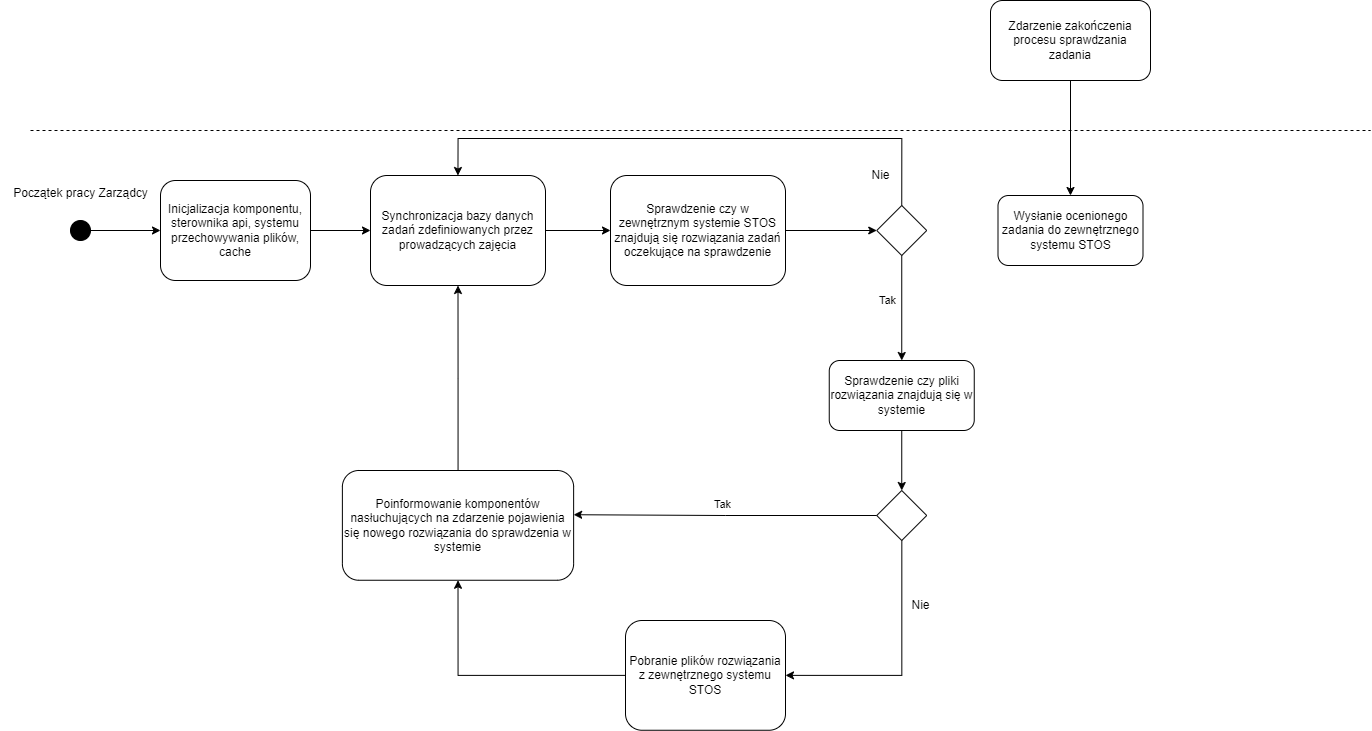
\includegraphics{img/3/zarzadca-diagram-aktywnosci.png}
		}
		\caption[Diagram aktywności zarządcy]{Diagram wizualizujący przebieg pracy zarządcy. Źródło własne.}
		\label{fig:scheduler-activity-diagram}
	\end{center}
\end{figure}

\subsection{Sterownik API}
Klasa sterownika API odpowiada za komunikację z zewnętrznym systemem STOS poprzez żądania HTTP do udostępnianego przez niego API, obejmującego takie punkty końcowe jak:
\begin{itemize}
    \item \textit{GET /sync} - pobranie wartości skrótu bazy danych
    \item \textit{GET /sync\_problem} - pobranie pliku bazy danych
    \item \textit{GET /tasks} - pobranie listy zadań oczekujących na sprawdzenie
    \item \textit{GET /files/<file\_id>} - pobranie pliku źródłowego zadania o danym id
    \item \textit{POST /tasks/<task\_id>} - przesłanie rozwiązania zadania o danym id
\end{itemize}
Interfejs sterownika API zawiera sygnatury metod służących do odpytywania każdego z punktów końcowych udostępnianych przez system STOS.
\lstset{style=python}
\begin{lstlisting}[caption = {Interfejs sterownika API.}]
    class IApiDriver(ABC):

    # Downloads files of available task
    @staticmethod
    @abstractmethod
    def fetch_tasks() -> StosTaskResponse:
        pass

    # Downloads file of given id
    @staticmethod
    @abstractmethod
    def download_file(id: str) -> tuple[str, str]:
        pass

    # Uploads score of a given task
    @staticmethod
    @abstractmethod
    def upload_results(id: str) -> None:
        pass

    # Downloads hash of files.db database
    @staticmethod
    @abstractmethod
    def fetch_remote_tag() -> StosRemoteTagResponse: 
        pass

    # Downloads zipped files.db database
    @staticmethod
    @abstractmethod
    def fetch_filesdb_zip() -> None:
        pass
\end{lstlisting}
Rządania są wykonywane przy użyciu biblioteki requests\cite{pythonRequests}, która w znacznym stopniu upraszcza wysyłanie rządań http w programach napisanych w języku Python.

\subsection{Sterownik systemu plików}
Interfejs sterownika systemu plików udostępnia dwie metody. Metoda \textit{save\_file} przyjmuje w argumentach nazwę, rozszerzenie oraz zawartość pliku i zapisuje go na dysku i zwraca ścieżkę do zapisanego pliku. Pliki zadań są potrzebne w systemie tylko na czas kompilacji i oceny, dlatego są zapisywane w folderze \textit{/tmp} przeznaczonym do przechowywania plików tymczasowych. Drugą metoda \textit{get\_file} służy do uzyskania zawartości pliku znajdującego się pod ścieżką podaną w argumencie metody.

\lstset{style=python}
\begin{lstlisting}[caption = {Interfejs sterownika systemu plików.}]
    class IStorageDriver(ABC):
    
    # Save file with filename and extension and return URL/PATH
    @staticmethod
    @abstractmethod
    def save_file(filename: str, content: str, extension: str) -> str:
        pass

    # Get contents of file under url. Returns None if file does not exist
    @staticmethod
    @abstractmethod
    def get_file(url: str) -> str | None:
        pass
\end{lstlisting}

\subsection{Sterownik cache}
Sterownik cache to element systemu mający zepewnić redukcję ilości wysyłanych rządań do systemu STOS, poprzez przechowywanie plików wchodzących w skład zadania, dzięki czemu po uzyskaniu listy plików zadań, pobierane są tylko te, które nie znajdują się obecnie w cache. Sam cache został zaimplementowany przy wykorzystaniu bazy danych SQLite\cite{sqlite}, czyli bazy danych przeprowadzającej operacje zapisu i odczytu bezpośrednio na pliku na dysku, bez wykorzystywania dodatkowych procesów serwera bazy danych. Rozwiązanie to zostało wybrane ze względu na jego prostotę oraz fakt, że jest to baza danych wykorzystywana w innych miejscach systemu. Interfejs sterownika cache udostępnia metody do dodawania, usuwania i pobierania plików oraz metodę \textit{check\_files}, która w argumencie przyjmuję listę nazw plików. Metoda ta sprawdza, czy w cache znajdują się pliki, których nazwy znajdują się na liście i zwraca listę z nawami tych, których brakuje.
\lstset{style=python}
\begin{lstlisting}[caption = {Interfejs sterownika systemu plików.}]
    class ICacheDriver(ABC):

    # Checks cache for existence of files and returns missing files
    @staticmethod
    @abstractmethod
    def check_files(files: list[str]) -> list[str]:
        pass

    # Adds entry regarding a single file to cache and overwrites old record
    @staticmethod
    @abstractmethod
    def add_entry(file: str, path: str) -> None:
        pass

    # Deletes a record representing file
    @staticmethod
    @abstractmethod
    def delete_entry(file: str) -> None:
        pass

    # Get file entry, returns None if file does not exist
    @staticmethod
    @abstractmethod
    def get_entry(file: str) -> TaskFile | None:
        pass
\end{lstlisting}



\section{Orkiestrator kontenerów}
Orkiestrator kontenerów to element systemu pośredniczący między kontenerami przeprowadzającymi kompilację i~sprawdzanie kodu, a~zarządcą. Zarządca przekazuje mu obiekty przechowujące informacje o~zadaniach otrzymanych z zewnętrznego systemu STOS-WEB, które są zapisywane do kolejki. W~drugiej kolejce przechowywane są obiekty powiązane z kontenerami gotowymi do sprawdzenia zadania. W~sytuacji, gdy zarówno kolejka zadań jak i~kolejka kontenerów nie są puste, pobierane są z nich elementy, a~zadanie zostaje zlecone do sprawdzenia przez kontener. Gdy kontener kończy pracę, pobierane są wyniki sprawdzonego zadania, następnie są one przekazywane do zarządcy, a~obiekt reprezentujący kontener trafia z powrotem do kolejki kontenerów.

\subsection{Cele}
Celem implementacji orkiestratora było umożliwienie zrównoleglenia najbardziej czasochłonnego procesu sprawdzania zadań, czyli kompilacji i~wykonania ich. Umożliwia to skalowanie horyzontalne tej części systemu, co pozwoli na uruchomienie większej ilości modułów sprawdzających podczas dużego obciążenia systemu. Dodatkowym atutem modułu jest również zmiana skryptów inicjujących działanie kontenerów napisanych w~języku Bash na kod napisany w~języku Python, co poprawia czytelność, ułatwia znajdowanie błędów, śledzenie przebiegu programu i~przyszły rozwój systemu.

\subsection{Implementacja}
Do implementacji modułu orkiestratora zostały użyte moduły pochodzące standardowej biblioteki Pythona. Interfejs został stworzony przy pomocy modułu Abstract Base Classes\cite{pythonAbc} i~zawiera sygnatury pięciu kluczowych metod dla funkcjonowania komponentu. 

\lstset{style=python}
\begin{lstlisting}[caption = {Interfejs orkiestratora kontenerów.}]
	class IScheduler(ABC):

    # initialize worker containers
    @abstractmethod
    def initialize_workers(self) -> None:
        pass
     
    # add task data to queue 
    @abstractmethod
    def register_new_task(self, task_data: TaskData) -> None:
        pass

    # method that manages the assignment of a task to a container
    @abstractmethod
    def manage_workers(self) -> None:
        pass

    # start processing task inside worker docker container
    @abstractmethod
    def process_task(self, task_data: TaskData, worker_id: str) -> None:
        pass

    # register callback function that is run on task finish
    @abstractmethod
    def register_task_completion_callback(self, callback: Callable[[TaskData, Path], None]) -> None:
        pass
\end{lstlisting}

\subsubsection{Inicjalizacja komponentu i~kontenerów modułu kompilującego}
Metoda \textit{initialize\_workers} odpowiada za inicjalizację kontenerów modułu kompilującego. Zaimplementowane działanie metody zaczyna się od pobrania dostępnych zasobów komputera z wykorzystaniem modułu subprocess\cite{pythonSubprocess}, przy pomocy którego wywoływane są polecenia \textit{nproc}\cite{linuxNproc} oraz \textit{free}\cite{linuxFree} systemu Linux, w~celu uzyskania informacji o~dostępnej ilości wątków procesora oraz pamięci RAM. Zasoby, które zostaną przydzielone do pracy pojedynczemu kontenerowi, są odczytywane z pliku zawierającego zmienne środowiskowe tworzonego systemu. Aby określić maksymalną liczbę instancji kontenerów modułu kompilującego, dostępne zasoby są dzielone przez zasoby przeznaczone do wykorzystania przez jeden kontener, po czym uzyskana liczba jest zaokrąglana w~dół do najbliższej liczby całkowitej. Następnie przygotowywana jest struktura katalogów dla każdego kontenera (rysunek \ref{fig:scheduler-directory-structure}). Tworzone są współdzielone foldery wejścia/wyjścia, potoki przez które zachodzi komunikacja z kontenerem oraz foldery zawierające zewnętrzne zależności takie jak skrypty kontrolujące pracę wewnątrz kontenera, kompilatory i~bilbioteki niezbędne do kompilacji zadań. Tworzenie katalogów i~potoków odbywa się przy pomocy modułu os\cite{pytohnOs}, pozwalającego na interakcję z funkcjami systemu operacyjnego. Zewnętrzne zależności są kopiowane do utworzonych katalogów z użyciem modułu shutil\cite{pythonShutil}, udostępniającego funkcje do wyższego poziomu operacji na plikach, takich jak rekursywne kopiowanie całych ścieżek z plikami.
\begin{figure}[!ht]
	\begin{center}
		\resizebox{1\textwidth}{!} {
			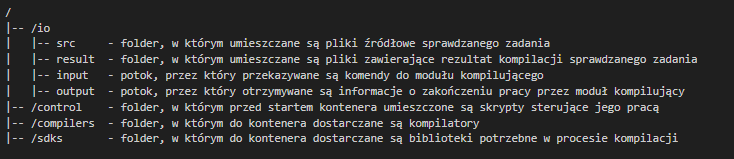
\includegraphics{img/3/orkiestrator-kontenerow-struktura-katalogow.png}
		}
		\caption{Struktura katalogów tworzona przy inicjalizacji modułu kompilującego. Źródło własne.}
		\label{fig:scheduler-directory-structure}
	\end{center}
\end{figure}
Ostatnim elementem inicjalizacji jest uruchomienie kontenerów poleceniem \textit{docker run} z obrazem \textit{wine-vs-runner} pozyskanym z obecnie funkcjonującego systemu STOS-WEB z argumentami:
\begin{itemize}
    \item \textit{--mount} -- powiązanie ścieżek systemu macierzystego z ścieżkami kontenera,
    \item \textit{--memory} -- ograniczenie zasobów pamięci RAM wykorzystywanej przez kontener,
    \item \textit{--cpus} -- ograniczenie zasobów procesora wykorzystywanych przez kontener,
    \item \textit{-d} -- uruchomienie kontenera bez blokowania terminala z kórego jest uruchamiany (\textit{detached}),
    \item \textit{--user} -- określenie użytkownika i~uprawnień kontenera.
\end{itemize}
oraz dodanie powiązanych z nimi obiektów do kolejki reprezentującej kontenery oczekujące na zlecenie zadania do sprawdzenia.

\subsubsection{Komunikacja z zarządcą}
Komunikacja z komponentem zarządcy odbywa się za pomocą wołań zwrotnych. Gdy zarządca otrzyma nowe zadanie, wywołuje metodę \textit{register\_new\_task} orkiestratora kontenerów, przekazując jej obiekt „TaskData” reprezentujący zadanie przesłane do sprawdzenia. Implementacja tej metody dodaje do kolejki obiekt przekazany w~argumencie. Komunikacja w~drugą stronę również odbywa się poprzez wołania zwrotne. Orkiestrator kontenerów udostępnia w~interfejsie metodę \textit{register\_task\_completion\_callback}, której argumentem jest funkcja przyjmująca obiekt sprawdzonego zadania oraz ścieżkę na dysku do plików rezultatu, której implementacja zapisuje w~liście przekazaną funkcję. Wszystkie funkcje z listy są wywoływane po sprawdzeniu zadania. Podejście to niesie za sobą korzyść zmniejszenia powiązania komponentów systemu. Umożliwia również, aby na zdarzenie sprawdzenia zadania nasłuchiwało wiele komponentów, mogą to być na przykład systemy logów, systemy tworzenia kopii zapasowych lub kilka instancji zarządców. Sprawia to, że system jest bardziej otwarty na rozbudowę o~nowe komponenty i~skalowanie.

\subsubsection{Przepływ zdarzeń orkiestratora kontenerów}
Orkiestrator kontenerów pozbawiony jest nieskończonej pętli aktywnie monitorującej stan i~wykonującj instrukcje. Zamiast tego jest sterowany zdarzeniami (rynsunek \ref{fig:scheduler-activity-diagram}), główna funkcja -- \textit{manage\_workers}, odpowiadająca za logikę biznesową wywoływana jest wtedy, gdy zmienia się stan kolejek zadań i~kontenerów. Implementacja metody sprawdza, czy w~zarówno w~kolejce zadań i~kolejce kontenerów znajdują się elementy, jeśli tak, pobiera po jednym elemencie i~rozpoczyna przetwarzanie zadania.

\begin{figure}[!ht]
	\begin{center}
		\resizebox{1\textwidth}{!} {
			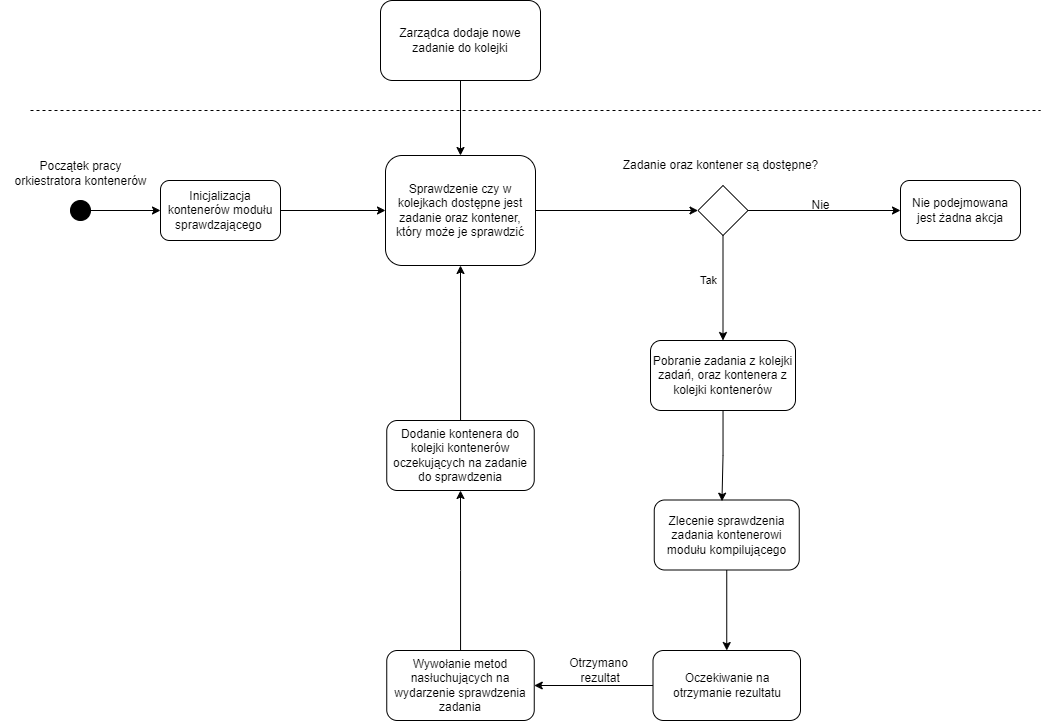
\includegraphics{img/3/orkiestrator-kontenerow-diagram-aktywnosci.png}
		}
		\caption[Diagram aktywności orkiestratora kontenerów]{Diagram wizualizujący przebieg pracy orkiestratora kontenerów. Źródło własne.}
		\label{fig:scheduler-activity-diagram}
	\end{center}
\end{figure}

Przetwarzanie zadania odbywa się wykonaniem metody \textit{process\_task}. Aby kontener modułu kompilującego mógł zacząć pracę, należy dostarczyć mu wszystkie pliki źródłowe przetwarzanego zadania skompresowane w~archiwum zip do katalogu \textit{io/src} katalogu współdzielonego. Archiwum tworzone jest modułem zipfile\cite{pythonZipfile}, zawierającym narzędzia do odczytu i~zapisu plików zip. Gdy archiwum znajduje się w~folderze, następuje wydanie polecenia do kontenera, poprzez wpisanie do potoku \textit{io/input} katalogu współdzielonego. Dostępne polecenia to:
\begin{itemize}
    \item \textit{vc-debug} - kompilacja w~trybie debugowania, generowane są dodatkowe informacje o~kodzie, zmiennych, funkcjach,
    \item \textit{vc-opt} - kompilacja z optymalizacją, w~procesie kompilacji poprawiana jest wydajność kodu wynikowego, może obejmować pominięcie zbędnych operacji, zmnianę struktury kodu, zmniejszenie rozmiaru plików wykonywalnych,
    \item \textit{vc-both} - kompilacja z optymalizacją w~trybie debugowania - połączenie poleceń vc-debug i~vc-opt.
\end{itemize}
Wydanie polecenia rozpoczyna proces kompilacji wewnątrz kontenera. Informacja o~zakończeniu kompilacji przekazywana jest poprzez potok \textit{io/output}, a~rezultat umieszczany jest w~katalogu \textit{io/result}. Orkiestrator kontenerów otwiera potok i~zapisuje go do zmiennej metodą \textit{open}, której argumentem jest ścieżka do potoku, a~następnie oczekuje na pojawienie się w~nim informacji i~odczyt metodą \textit{read}, która oprócz potoku przyjmuje w~argumencie maksymalną ilość odczytanych bajtów. Obie metody pochodzą z modułu os\cite{pytohnOs}. Po otrzymaniu informacji zwrotnej od kontenera, rezultat jest kopiowany do tymczasowego folderu przechowującego wyniki zadań, a~orkiestrator wywołuje wszystkie funkcje nasłuchujące na zdarzenie sprawdzenia zadania, przekazując im obiekt zadania oraz ścieżkę do skopiowanego rezultatu.

\lstset{style=python}
\begin{lstlisting}[caption = {Implementacja metody odczytującej informacje z potoku.}]
    # Wait for worker result 
    def watch_output_pipe(self, task_data: TaskData, worker_id: str) -> None:
        path = f'./worker_{worker_id}/io/output'
        if not os.path.exists(path):
            self.__stos_logger.error(f"watch_output_pipe: Path {path} does not exist.")
            return
        output_pipe = os.open(path, os.O_RDONLY)
        self.__stos_logger.info(f"watch_output_pipe: Waiting for task: {task_data.task_id} result from worker: {worker_id}")
        data = os.read(output_pipe, 1024)
        self.__stos_logger.info(f"watch_output_pipe: Result: {data} for task: {task_data.task_id} from worker: {worker_id}")
        os.close(output_pipe)
\end{lstlisting}

\subsubsection{Współbieżne przetwarzanie zadań}
W celu umożliwienia sprawdzania kilku zadań jednocześnie, dzieje się to w~sposób współbieżny. Python udostępnia narzędzia do tworzenia współbieżnych programów w~module threading\cite{pythonThreading}, zawierający wysokopoziomowe metody do zarządzania wątkami. Utworzone w~ten sposób wątki nie są jednak wykonywane równolegle, czyli w~danym momencie czasu wykonywana jest tylko instrukcja pochodząca z kodu jednego wątku programu, ale pozwala na wykonywanie innych operacji w~czasie oczekiwania na pojawienie się rezultatu zadania sprawdzanego przez kontener modułu kompilującego. Dzieje się tak ze względu na implementację interpretera Python, zawierającego w~sobię globalną blokadę interpretera (\textit{Global Interpreter Lock}\cite{pythonGlobalInterpreterLock}) zapobiegającą takiemu zachowaniu. Upraszcza to proces zarządzania sekcjami krytycznymi, czyniąc wiele operacji bezpiecznymi z perspektywy wykonywania współbieżnego bez zastosowania dodatkowych mechanizmów bezpieczeństwa, jednak tym samym nie wykorzystuje w~pełni możliwości wielordzeniowych procesorów. Aby zrównoleglić wykonywane operacje, należy wyłączyć globalną blokadę interpretera, budując go z kodu źródłowego z włączoną opcją \textit{--disable-gil} lub skorzystać z modułu multiprocessing\cite{pythonMultiprocessing}, który tworzy osobne procesy systemowe. W~implementacji orkiestratora kontenerów zastosowano moduł threading wraz ze standardowymi ustawieniami globalnej blokady interpretera, ponieważ ten komponent nie wykonuje skomplikowanych i~czasochłonnych operacji, a~jedynie odpowiada za zarządzanie kontenerami i~przepływ danych między nimi a~resztą systemu, więc wykonywanie go równolegle nie przyniosłoby wymiernego przyspieszenia działania systemu -- to etap kompilacji, który odbywa się w~kontenerach, jest najbardziej czasochłonny i~to własnie ten etap został zrównoleglony dzięki przeprowadzaniu go w~wielu instancjach kontenerów.

Nowe wątki są tworzone w~implementacji metody \textit{manage\_workers}, która sprawdza, czy w~kolejkach znajdują się zadanie oraz kontener, który mógłby je przetworzyć, a~następnie tworzy nowy wątek odpowiedzialny za przetworzenie zadania. Mimo że pojedyncze operacje na kolejkach pochodzących z modułu queue\cite{pythonQueue} sa bezpieczne wielowątkowo, to w~metodzie występuje sekcja krytyczna składająca się z kolejnego sprawdzenia stanu i~pobrania elementów z kolejki. Aby zapobiec sytuacji, w~której wykonanie funkcji w~jednym wątku sprawdzi, że kolejki nie są puste i~wejdzie do bloku warunkowego, a~inny wątek w~tym czasie pobierze element z kolejki, zastosowano mechanizm semafora binarnego, uniemożliwiającego wielu wątkom jednoczesne wykonywanie kodu znajdującego się w~sekcji krytycznej.

\lstset{style=python}
\begin{lstlisting}[caption = {Implementacja metody rozpoczynającej przetwarzanie zadania.}]
    @override
    def manage_workers(self) -> None:
        with self.__lock:
            while not self.__workers_queue.empty() and not self.__tasks_queue.empty():
                task = self.__tasks_queue.get()
                workerId = self.__workers_queue.get()
                thread = threading.Thread(target=self.process_task, args=(task, workerId))
                thread.start()
\end{lstlisting}

\section{Moduł kompilujący}
W czasie prac nad projektem nie była dostępna istniejąca część systemu modułu kompilującego, odpowiedzialnego za kompilację kodu. Znane były funkcjonalności oraz wymagania, które musiał spełniać ten moduł, co pozwoliło na implementację własnego modułu. Rozwiązanie w~obecnym stanie było używane jedynie do testów, jednak jest otwarte na modyfikacje i~dalszy rozwój w~przyszłości. W~tym rozdziale zostanie opisany zaimplementowany przez nas moduł, a~nie zintegrowany w~ostatecznym rozwiązaniu kontener pochodzący z obecnego systemu STOS-SERVICE. Na etapie projektowania i~implementacji nie był znany dokładny interfejs obrazu istniejącego kontenera, przez co nie jest on z nim kompatybilny. 

\subsection{Wymagania}
Otrzymane wymagania do modułu kompilującego obejmowały wykorzystane technologie oraz sposób działania. Moduł musiał być skonteneryzowany, zapewniając izolację wykonywanego kodu zadania od systemu operacyjnego i~procesów systemu macierzystego. Ze względu na dostępność wiedzy, łatwość implementacji oraz utrzymywania systemu, oprogramowaniem służącym do konteneryzacji miał być Docker. Został również określony wymóg, aby czas wykonania zadania był niezależny od obciążenia i~dostępnej mocy obliczeniowej systemu macierzystego. Dodatkowo system miał zapewniać wykonywanie programu zadania tak, jakby był wykonywany na maszynie z systemem operacyjnym Windows. Ważnym aspektem był również niski koszt związany z potencjalną awarią i~ponownym przywróceniem działania tej części systemu.

\subsection{Obraz bazowy}
Wybranym obrazem bazowym do kontenera zostało Ubuntu 20.04\cite{linuxUbuntu}, jest to popularny wybór, dzięki czemu jest dobrze przetestowany i~kompatybilny z wieloma narzędziami. Obrazy Ubuntu dostępne w~Docker Hub to systemy oparte na Ubuntu Base, czyli lżejszej wersji Ubuntu, nieposiadającej oprogramowania, które nie jest przydatne do pracy w~kontenerze takich jak interfejs graficzny lub aplikacje biurowe. Wersja 20.04 jest wersją Long-Term Support, co oznacza, że przez długi czas oferuje aktualizacje bezpieczeństwa oraz poprawki. Posiada również bogate repozytorium pakietów, oferujące wszystkie potrzebne w~naszym zastosowaniu narzędzia.

\subsection{Wykorzystane pakiety}
Wszystkie pakiety konieczne do prawidłowej pracy kontenera zostały pozyskane z repozytorium Ubuntu 20.04 przy pomocy systemu zarządzania pakietami apt-get. Obejmowały kompilator mingw, narzędzie Wine pozwalające na uruchamianie aplikacji przeznaczonych na system operacyjny Windows oraz wirtualny serwer Xvfb zapewniający wirtualne środowisko graficzne dla Wine.

\subsection{Wymiana plików między kontenerem a~systemem macierzystym}
Narzędzie Docker zapewnia dwie podstawowe metody wymiany plików między kontenerem a~systemem macierzystym -- Docker Volume\cite{dockerVolume} oraz Bind mounts\cite{dockerBindMounts}. Docker Volume jest mechanizmem zarządzanym przez system Docker, odpowiada on za tworzenie, zarządzanie i~usuwanie danych. Możliwe jest współdzielenie jednego wolumenu przez liczne kontenery. Bind mounts to prostsze rozwiązanie polegające na bezpośrednim połączeniu wybranego katalogu w~systemie macierzystym z katalogiem kontenera. Zapewnia to większą elastyczność, ponieważ nie wymaga tworzenia osobnego wolumenu, a~jedynie powiązania ścieżki bezwzględnej na systemie macierzystym, ze ścieżką wewnątrz kontenera, jednak tym samym zmniejsza to izolację kontenera od systemu. W~naszym rozwiązaniu zostały wykorzystane bind mounts, ponieważ każde sprawdzane rozwiązanie otrzymuje swój osobny folder powiązany z jego unikalnym id, który wiążemy z osobnym, nowo utworzonym kontenerem. Eliminuje to potrzebę zarządzania licznymi wolumenami lub dzielenia wolumenu między kilka kontenerów co z kolei zmniejszyłoby izolację między zadaniami. Aby zaimplementowany kontener poprawnie skompilował i~uruchomił program, struktura powiązanego folderu powinna wyglądać w~następujący sposób:
\dirtree{%
.1 folder powiązany.
.2 source.
.3 main.cpp.
.2 input.
.3 1.in.
.3 2.in.
.3 n.in.
.2 output.
.3 1.out.
.3 2.out.
.3 n.out.
}
W katalogu \textit{/source} znajdują się pliki zawierające kod źródłowy C++. Wejście, które chcemy przekazać przy uruchamianiu programu, znajduje się w~plikach *.in w~folderze \textit{/input}. W~trakcie działania programu tworzone są pliki wynikowe z rozszerzeniem *.out w~folderze \textit{/output}. 

\subsection{Skrypt uruchamiany przy starcie kontenera}
Punkt wejścia to skrypt wskazany w~pliku Dockerfile, który uruchamia się po starcie kontenera. Został napisany w~Bashu i~realizuje funkcjonalność modułu kompilującego, kompiluje pliki *.cpp znajdujące się w~katalogu \textit{/source} powiązanego folderu za pomocą mingw, a~następnie uruchamia skompilowany program dla każdego z plików wejścia *.in umieszczonych w~folderze \textit{/in}. Wynik każdego uruchomienia przekierowywany jest do pliku wynikowego *.out w~folderze \textit{/out} katalogu współdzielonego. Każde uruchomienie dodatkowo mierzy czas wykonania przy pomocy komendy date.
\begin{figure}[!ht]
	\begin{center}
		\resizebox{1\textwidth}{!} {
			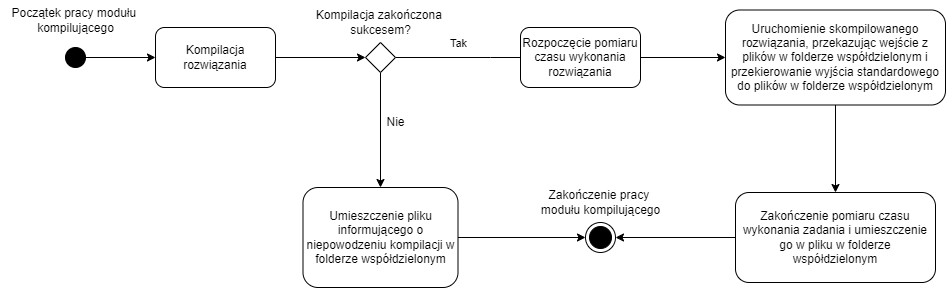
\includegraphics{img/3/diagram-aktywnosci-modul-kompilujacy.png}
		}
		\caption[Diagram aktywności modułu kompilującego]{Diagram wizualizujący przebieg pracy modułu kompilującego. Źródło własne.}
		\label{diagram-aktywnosci-worker}
	\end{center}
\end{figure}

\subsection{Ograniczenie zasobów kontenera}
Jednym z elementów zapewnienia sprawiedliwej oceny czasu wykonania zadania jest określenie maksymalnej ilości pamięci ram oraz zasobów procesora, które są dostępne dla kontenera. Domyślnie kontener nie posiada żadnych ograniczeń wykorzystywanych zasobów i~wykorzystuje ich tyle, ile zostanie mu przydzielone przez jądro systemu macierzystego. Te wartości można jednak ograniczyć, korzystając z mechanizmu kontroli maksymalnych zasobów wykorzystanych przez kontener udostępnionego przez narzędzie Docker\cite{dockerConstraints}, poprzez użycie flag --memory oraz --cpus przy starcie kontenera. Zakładając, że przydzielone kontenerom zasoby nie przekraczają całości dostępnych zasobów komputera, możemy osiągnąć względnie sprawiedliwą ocenę czasu wykonania zadania. Rozwiązaniem, które pozwala z większą dokładnością określić zasoby czasowe potrzebne do wykonania programu, jest pomiar wykorzystania procesora na podstawie liczby cykli, jednak implementacja tej funkcjonalności wewnątrz kontenera Dockerowego wiąże się z koniecznością uruchomienia go ze zwiększonymi uprawnieniami do funkcji jądra, co znacząco zmniejsza izolację modułu i~bezpieczeństwo całego systemu, w~szczególności biorąc pod uwagę fakt, że moduł ten odpowiada za kompilację i~wykonanie potencjalnie szkodliwego kodu przesłanego przez użytkowników zewnętrznego systemu STOS.

\subsection{Różnice w~funkcjonowaniu aplikacji na systemach Windows i~Linux}
\subsubsection{Linux}
Systemy Linux to systemy bazujące jądrze Linux. Jądro to zostało udostępnione w~1991 przez Linusa Torvaldsa na licencji GNU General Public License, co oznacza, że jego kod źródłowy jest publicznie dostępny, a~użytkownicy mają wolność do uruchamiania, analizowania, rozpowszechniania i~udoskonalania programu.
Jest systemem uniksopodobnym i~zgodny ze standardem POSIX, czyli jego monolityczna budowa jądra, model systemu plików, komunikacja międzyprocesowa, zarządzanie pamięcią, interfejs programistyczny i~użytkownika są zbliżone do systemu Unix, jednak jego kod źródłowy nie wywodzi się z kodu źródłowego Uniksa. Struktura katalogów w~systemie Linux jest zdefiniowana w~Filesystem Hierarchy Standard\cite{linuxFhs} i~składa się z katalogu głównego, w~którym znajdują się wszystkie inne katalogi, bazowo takie jak:
\begin{verbatim}
    /root
    |-- /bin/ - podstawowe pliki wykonynwalne (binaries)
    |-- /boot/ - pliki rozruchowe
    |-- /dev/ - pliki urządzeń
    |-- /etc/ - pliki konfiguracyjne
    |-- /tmp/ - pliki tymczasowe
    |-- /lib/ - biblioteki współdzielone
    |-- /var/ - pliki, których zawartość często ulega zmianie (np. logi)
    |-- /usr/ - pliki współdzielone i~niezmienne
    |-- /home/ - pliki użytkownika
\end{verbatim}

\subsubsection{Windows}
Systemy Windows to systemy wyprodukowane przez firmę Microsoft, które od 1993 bazują na hybrydowym jądrze\cite{windowsHybridKernel} NT (New Technology)\cite{windowsNT} zawierające między innymi funkcje jak zarządzania procesami, pamięcią, urządzeniami, przerwaniami systemowymi, komunikacją między procesową. Hybrydowość jądra oznacza, że posiada ono jednocześnie cechy jądra monolitycznego oraz mikrojądra, w~jądrze NT działa to na zasadzie przestrzeni jądra oraz przestrzeni użytkownika. Przestrzeń jądra ma pełny dostęp do zarządzania pamięcią, procesami, systemem plików oraz urządzeń, a~przestrzeń użytkownika to przestrzeń, w~której te dostępy są ograniczone, a~operacje dostępu do zasobów systemowych odbywają się, korzystając z interfejsu systemowego jądra, poprzez wołania systemowe. Taki podział ma na celu zwiększenie bezpieczeństwa i~zmniejszenie podatności na awarię systemu. Domyślnym systemem plików w~systemach bazujących na jądrze NT jest NTFS, w~którym dyski rozdzielone są na partycje systemowe.

\subsubsection{Wpływ różnic na wykonanie aplikacji w~obu systemach}
Różnice między systemem Linux a~Windows są widoczne na każdym aspekcie, począwszy od jądra, systemu plików, wydajności, licencjonowania, dostępnego oprogramowania. Przekładają się na działanie aplikacji w~tych systemach. Komunikacja programu z systemem operacyjnym jest oparta na innych, niekompatybilnych ze sobą interfejsach, oba systemy bazują na innych systemach plików. Aplikacje w~systemie Windows korzystają z dynamicznie ładowanych systemowych bibliotek, a~swoje ustawienia i~konfiguracje często zapisują w~rejestrze systemowym. Linuksowe odpowiedniki bibliotek .dll jako pliki .so oraz sposób zapisywania konfiguracji aplikacji w~katalogu \textit{/etc} nie są kompatybilne z Windowsem. Sprawia to, funkcjonowanie aplikacji, jak i~proces kompilacji oraz wykonania kodu C++ różni się między dwoma systemami.

\subsection{Uruchamianie aplikacji przeznaczonych na system operacyjny Windows na systemie operacyjnym Linux}
\subsubsection{Emulator i~warstwa kompatybilności}
Emulator to oprogramowanie tworzące wirtualną maszynę innej platformy. Uruchamianie aplikacji na emulatorze, nie różni się od uruchamiania jej na natywnej platformie, symulowany jest cały system docelowy. Wadą stosowania emulatora jest nieporównywalnie gorsza wydajność w~porównaniu do natywnej platformy. W~artykule\cite{emulatorPerformance} porównującym wydajność emulatorów Android Studio oraz Blue Stacks do urządzeń fizycznych z systemem Android, uzyskano od trzech, do nawet dwudziestu pięciu razy gorszą wydajność w~aplikacji testowej polegającej na wykonaniu algorytmu szachowego mini-max. Warstwa kompatybilności również pozwala na uruchomienie aplikacji zaprojektowanej na inną platformę, jednak zamiast przeprowadzać kosztowną symulację całego systemu docelowego, zamienia ona wołania systemowe pochodzące z uruchamianego programu na te z systemu macierzystego, dzięki czemu aplikacja działa tak, jak działałaby na natywnej platformie, a~system macierzysty otrzymuje właściwe dla siebie żądania. Dzięki braku konieczności symulowania całej maszyny warstwa kompatybilności zapewnia lepszą wydajność od emulatora i~nie wymaga dużego nakładu pamięci.

\subsubsection{Wine\cite{wine}}
Wine to warstwa kompatybilności aplikacji przeznaczonych do wykonywania na systemie Windows na systemach zgodnych ze standardami POSIX, takich jak Linux, macOS. Jest oprogramowaniem open source, który jest wciąż aktywnie wspierany przez społeczność oraz firmę CodeWeavers, a~jego pierwsza wersja została wydana w~1993 roku. Ze względu na to, że ponad 70\% komputerów osobistych korzysta z systemów operacyjnych Windows\cite{windowsMarketShare}, programy użytkowe takie jak aplikacje biznesowe, narzędzia biurowe czy gry komputerowe często tworzone są tylko na tę platformę, co może ograniczać użytkownikom możliwość wyboru używanego systemu, prowadzić do monopolu i~wymuszać zakup licencji Windows. Wine oraz inne programy realizujące podobną funkcjonalność, pozwalają na wybór preferowanego systemu, bez rezygnowania z dostępu do puli programów nieoferujących wsparcia dla niego.

\begin{figure}[!h]
	\begin{center}
		\resizebox{1\textwidth}{!} {
			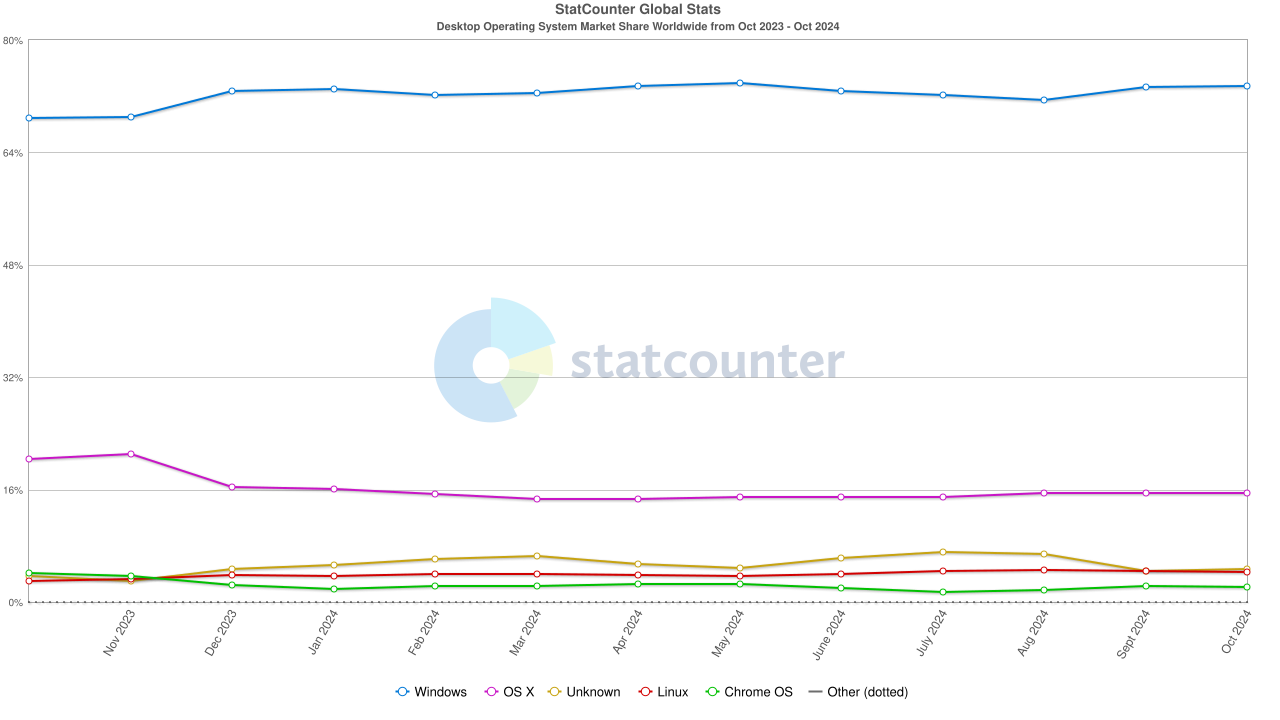
\includegraphics{img/3/desktop-os-market-share.png}
		}
		\caption{Wykres przedstawiający udział systemów operacyjnych wśród komputerów osobistych. Źródło: https://gs.statcounter.com/os-market-share/desktop/worldwide/.}
		\label{desktop-os-market-share}
	\end{center}
\end{figure}

Wine podczas pracy korzysta z folderu zawierającego wirtualne środowisko -- Wineprefix\cite{wineprefix}, gdzie znajdują się pliki symulujące system Windows. Są tam pliki rejestrów, biblioteki, pliki konfiguracyjne oraz struktura folderów odpowiadająca podziałowi na partycje systemowe systemu Windows, które tworzone jest domyślne przy instalacji programu. Użytkownik może utworzyć więcej środowisk, z dostosowanymi ustawieniami architektury, narzędzi, bibliotek dll czy wersji systemu, oraz zmieniać wykorzystywane obecnie środowisko. Konfiguracja środowiska odbywa się przy pomocy narzędzia Winetricks\cite{winetricks}. Izoluje to działanie programu od wirtualnego środowiska i~umożliwia jego konfigurację do własnych potrzeb. Aby uruchomić program przy pomocy Wine, należy uruchomić go za pomocą komendy:
\begin{verbatim}
wine <plik wykonywalny>
\end{verbatim} Wine ładuje program do pamięci, parsuje go, dołącza potrzebne zależności i~przechodzi do wykonywania programu. Gdy w~trakcie pracy programu pojawi się wołanie systemowe, Wine przechwytuje je i~zamienia na zgodne ze standardami POSIX. 

Wine jako projekt otwartoźródłowy jest bazą licznych alternatyw\cite{wineBasedProjects} z których najbardziej zaawansowanymi są Proton\cite{proton} oraz CrossOver\cite{crossover}. CrossOver to płatne oprogramowanie firmy CodeWeavers, czyli firmy, która również zajmuje się rozwojem projektu Wine. W~odróżnieniu od Wine, CrossOver zapewnia graficzny interfejs użytkownika. Dodatkowo rozwój Wine jest bardziej restrykcyjny i~czasochłonny -- nowe funkcjonalności muszą zostać zaimplementowane w~sposób zgodny z określonymi standardami, tak, aby tłumaczenie wołań systemowych odbywało się w~jak najdokładniejszy sposób. W~przypadku CrossOver rozwój stawia bardziej na aspekty użytkowe -- w~celu szybszego naprawienia problemu występującego w~aplikacji często używanej przez użytkowników programu, twórcy mogą wprowadzić zmiany specyficzne dla danej aplikacji, aby ten konkretny problem nie występował. Z czasem może to zostać naprawione w~sposób należyty w~wersji Wine, które to są regularnie integrowane do kodu źródłowego CrossOver.

Proton opracowywany jest przez Valve, realizuje podobną funkcjonalność, jednak jego rozwój jest skupiony na zapewnieniu poprawnego działania platformy Steam oraz gier przeznaczonych na tę platformę w~systemie Linux poprzez warstwę kompatybilności między programistycznym interfejsem przeznaczonym na systemy Windows -- Direct3D, służącym do rysowania trójwymiarowych obiektów, na wieloplatformowy odpowiednik -- Vulkan.


% LTex: language=pl
\chapter{Wdrożenie}

% --------------
% Serwer fizyczny
% -------------

% LTex: language=pl
\section{Serwer fizyczny}
W ramach przebudowy istniejącego systemu STOS zostały zakupione 2 nowe serwery fizyczne w~ramach przetargu rozpisanego przez Politechnikę Gdańską, na które miał zostać wdrożony system STOS.

\subsection{Komponenty serwera}
Każdy z tych serwerów zbudowany jest oparty na architekturze AMD64 i~korzysta z chipsetu AMD X670 i~gniazda procesora zgodnego ze specyfikacją AM5 oferowanych przez płytę główną GIGABYTE X670 Gaming v2 \cite{gigabyteX670}. Jako procesor wykorzystano kompatybilny z płytą główną procesor AMD Ryzen 9 7950X, posiadający 16 rdzeni i~32 wątki o~bazowym taktowaniu zegara o~częstotliwości $4,5 Ghz$ i~taktowaniem maksymalnym $5,7 Ghz$ \cite{ryzen}. Wspiera on maksymalnie $128 GB$ pamięci RAM w~standardzie DDR5, w~tym serwerze zainstalowano zestaw 4 kości, każda o~pojemności $32 GB$, składające się na zestaw Patriot Viper Venom 128GB DDR5, z taktowaniem $6400 Mhz$ i~opóźnieniem CAS wynoszącym 32 cykle zegara (CL32) \cite{patriotRam}. Za chłodzenie procesora odpowiada chłodnica Shadow Rock 3 produkowana przez firmę CoolerMaster, wykorzystująca mechanizm chłodzenia powietrznego \cite{coolermaster}. Na pamięć trwałą serwera składają się 3 dyski, 2 dyski w~technologii M.2 Samsung Evo 990 o~pojemności $1 TB$ każdy \cite{samsungSsd}, i~dysk SSD Silicon Ace A55 \cite{sataSsd} o~pojemności $4 TB$, łącznie dające $6 TB$ pamięci trwałej. System zasilany jest zasilaczem Gigabyte UD1000GM PG5, certyfikowanym standardem 80+ Gold i~charakteryzującym się dostarczaną mocą w~wysokości $1 kW$ \cite{zasilka}.  Obudową serwera jest obudowa Silver Monkey X Fence SMXC008 z wbudowanym wentylatorem o~średnicy 120 mm \cite{obudowa}.

\subsection{Potencjalne wady konfiguracji sprzętowej}
Pierwszym potencjalnym problemem wynikającym z powyższej specyfikacji sprzętowej jest ograniczenie możliwej do wykorzystania pamięci RAM narzucone przez procesor. W~razie potrzeby zwiększenia dostępnej pamięci operacyjnej na serwerze konieczna jest również wymiana procesora na taką jednostkę, która pozwala na skorzystanie z takiej, większej, ilości pamięci. Kolejnym potencjalnym wąskim gardłem jest zastosowane rozwiązanie chłodzenia procesora. Chłodnica wykorzystana w~serwerze, CoolerMaster Shadow Rock 3, według specyfikacji, jest w~stanie skutecznie utrzymać akceptowalną temperaturę procesora o~mocy do $190 W$, wyrażanej jako TDP (Thermal Design Power), oznaczająca maksymalne zużycie mocy przez komponent, w~tym przypadku procesor, które należy brać pod uwagę przy projektowaniu systemu \cite{intelTdp}. AMD Ryzen 7950X, przy bazowym taktowaniu zegara, szacowany jest przez producenta na charakteryzujący się mocą $170 W$ TDP. Sam zapas $20W$ jest wystarczający w~przypadku chłodzenia procesora, lecz w~przypadku Ryzena 7950X pracującego w~trybie boost, jego zużycie energii jest w~stanie dochodzić do ok. $230 W$ - $250 W$ \cite{amdPpt, testyMocy}, co jest równoznaczne z deficytem mocy chłodnicy rzędu od $40W$ do $60W$. Zastosowanie obecnego chłodzenia może, z dużym prawdopodobieństwem, doprowadzić do powstania efektu znanego jako „thermal throttling” \cite{throttling}. Polega on na ograniczaniu mocy i~prędkości procesora, gdy osiąga on temperatury dochodzące do maksymalnych dopuszczalnych przez producenta temperatur, mieszczących się zazwyczaj w~zakresie od $95^{\circ}\mathrm{C}$ do $105^{\circ}\mathrm{C}$. W~przypadku powyższej konfiguracji, efekt ten powstawać będzie przy zwiększonym obciążeniu serwera, uniemożliwiając procesorowi wykorzystanie w~pełni jego potencjału taktowania. Dodatkowym czynnikiem jest stosunkowo niska objętość powietrza odprowadzanego ze środka obudowy serwera, za którą odpowiedzialny jest jeden wiatrak o~średnicy 120 mm. Warto nadmienić, że są to jedynie rozważania teorytyczne i~w~celu ustalenia faktycznej wydajności zastosowanego chłodzenia, należałoby przeprowadzić odpowiednie testy serwera, które nie znajdują się w~zakresie tego projektu.

\begin{figure}[!h]
	\begin{center}
		\resizebox{0.7\textwidth}{!} {
			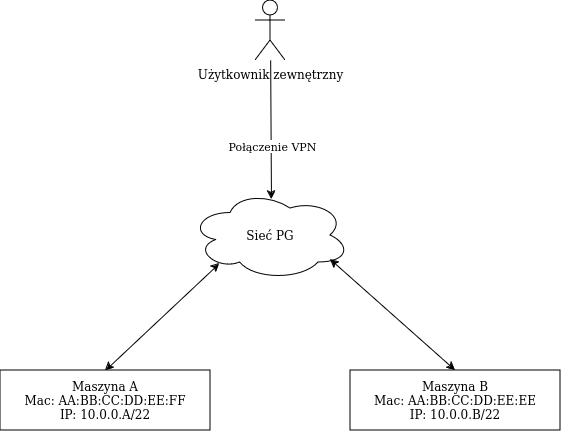
\includegraphics{img/4/fizycznaSiec.png}
		}
		\caption[Diagram fizycznego rozmieszczenia maszyn w~sieci Politechniki Gdańskiej]{Diagram przedstawiający umiejscowienie maszyn fizycznych w~sieci Politechniki Gdańskiej. Adresy IP i~adresy MAC nie są faktycznymi adresami maszyn w~sieci. Źródło własne.}
		\label{diagramSiecFizyczna}
	\end{center}
\end{figure}

\subsection{Serwery w~kontekście sieci Politechniki Gdańskiej}
Obie maszyny fizyczne znajdują się na terenie Politechniki Gdańskiej i~znajdują się w~sieci wewnętrznej PG. Posiadają one statycznie przypisane z poziomu sieci adresy IP, odpowiadające adresom MAC ich kart sieciowych. Dostęp z sieci zewnętrznych odbywa się za pomocą VPN Politechniki Gdańskiej i~uzyskaniu dostępu do sieci politechnicznej. Topologię maszyn fizycznych w~kontekście sieci przedstawia diagram \ref{diagramSiecFizyczna}.



% --------------
% Kubernetes
% -------------

% LTex: language=pl
\section{Koncepcja wdrożenia jako klaster Kubernetes}
Aby efektywnie wykorzystać wcześniej wspomniane mechanizmy ograniczania wykorzystywanych zasobów sprzętowych, pierwsza koncepcja architektury wdrożenia systemu była oparta na orkiestratorze kontenerów Kubernetes, systemie pozwalającym na zautomatyzowane wdrażanie, skalowanie i~zarządzanie potencjalnie wysoką liczbą kontenerów\cite{k8sMain}.

\subsection{Orkiestratory kontenerów}
Wraz ze wzrostem popularności architektur aplikacji opartych na mikroserwisach, wzrosła również podaż na systemy pozwalające na zarządzanie, monitorowanie i~skalowanie instancji poszczególnych serwisów aplikacji wdrożonych na wielu maszynach fizycznych, szczególnie w~dużych systemach komercyjnych. Odpowiedzią rynku wypełniającą tę lukę są systemy orkiestracji kontenerów. Dwoma najpopularniejszymi orkiestratorami na rynku są Kubernetes i~Docker Swarm.

\subsubsection{Docker Swarm}
Docker Swarm to rozwiązanie wbudowane bezpośrednio w~silnik Dockera, pozwalające na stosunkowo proste wdrożenie złożonych aplikacji\cite{dockerSwarm}. Zawiera podstawowe funkcjonalności orkiestratora, takie jak wdrażanie aplikacji za pomocą plików konfiguracyjnych (korzysta ze standardu Docker Compose\cite{dockerCompose}), monitorowanie stanu serwisów oraz obsługę wdrożenia na kilku maszynach fizycznych. Niewątpliwą zaletą tego rozwiązania jest jego prostota i~stosunkowo niski próg wejścia dla użytkowników zaznajomionych z technologią Docker i~Docker Compose, co pozwala na uniknięcie kosztów związanych ze szkoleniem administratora systemu. Jednakże prostota ta wiąże się również z ograniczeniem możliwości konfiguracji takiego systemu, a~dość niska popularność Docker Swarm w~porównaniu do Kubernetes niesie za sobą koszty związane z samodzielną implementacją pewnych rozwiązań, których odpowiedniki w~technologii Kubernetes są dostępne za darmo i~utrzymywane przez społeczność.
\subsubsection{Kubernetes}
Kubernetes to rozwiązanie, z którego korzystają największe projekty komercyjne\cite{googleKubernetes}, początkowo rozwijane przez firmę Google. Sam system Kubernetes dostępny jest, podobnie jak system operacyjny Linux, w~postaci różnych dystrybucji. Spółki oferujące usługi chmurowe dla klientów, takie jak Amazon i~Google, często decydują się na rozwój własnych dystrybucji Kubernetesa, lecz istnieją również dystrybucje przeznaczone dla mniejszych projektów, takie jak MicroKubernetes\cite{microk8s}, który został wykorzystany podczas prototypowania rozwiązania wdrożenia systemu STOS. Kubernetes posiada bogaty ekosystem i~wbudowane rozwiązania, pozwalające na znaczące uproszczenie konfiguracji wirtualnej sieci, w~której znajduje się wdrażany system. Rozwiązanie to, w~przeciwieństwie do Docker Swarm, jest niezależne od zastosowanej technologii konteneryzacji, pozwalając na używanie więcej niż jednej technologii w~ramach jednego klastra. Dodatkowo Kubernetes wspiera menadżera pakietów/zasobów w~postaci programu Helm\cite{k8sHelm}, dzięki czemu dostępnych jest wiele darmowych rozwiązań utrzymywanych przez społeczność, pozwalających między innymi na automatyczne gromadzenie logów i~monitorowanie poszczególnych serwisów wdrożonych w~systemie. Podobnie jak w~przypadku Docker Swarm, stopień skomplikowania Kubernetesa stanowi jego największą zaletę i~wadę. Przez wysoki próg wejścia, administracja systemem, a~w~szczególności jej nauka, stanowi czasochłonny proces. Podobnie jest w~przypadku utrzymania, dla osób niezaznajomionych z Kubernetesem i~jego poszczególnymi elementami, diagnostyka potencjalnych problemów i~ich naprawa staje się nieporównywalnie trudniejszym zadaniem niż w~przypadku Docker Swarm. Jednakże, rozwiązanie wdrożone na bazie klastra Kubernetes oferuje o~wiele więcej możliwości potencjalnego rozwoju systemu, zarówno pod względem bardziej rozbudowanej architektury jak i~wdrażania dodatkowych rozwiązań monitorowania.

\subsection{Wybór orkiestratora}
Mając na uwadze wady i~zalety rozwiązań opartych o~MicroKubernetes i~Docker Swarm, podjęto decyzję o~początkowym rozwoju rozwiązań opartych o~obie z tych technologii. Faktycznie, wdrożenie samej aplikacji za pomocą Docker Swarm zajęło zauważalnie mniej czasu niż w~przypadku MicroKubernetesa (osoba wdrażająca nie miała wcześniejszego doświadczenia z żadnym z tych systemów). Przy próbie wdrożenia rozwiązania pozwalającego na monitorowanie logów systemu, prawidłowość ta prezentowała się zgoła odwrotnie -- dzięki menadżerowi pakietów Helm, wdrożenie tzw. „stacka ELK” (czyli aplikacji Elasticsearch, Logstash i~Kibana) na klastrze MicroKubernetes odbyło się nieporównywalnie szybciej niż w~przypadku Docker Swarm, który wymagał ręcznej konfiguracji poszczególnych kontenerów odpowiedzialnych za każdy z serwisów wchodzących w~skład rozwiązania zbierającego logi z systemu. Na podstawie doświadczeń związanych z utrudnionym wdrożeniem zewnętrznych systemów na klastrze Docker Swarm i~możliwych przyszłych komplikacjach przy konieczności dodawania kolejnych serwisów do klastra, podjęto decyzję o~kontynuowaniu prac z MicroKubernetesem.

\subsection{Prototyp wdrożenia i~jego zalety}
Z perspektywy administratorów systemu STOS i~pracowników katedry, którzy w~przyszłości będą utrzymywać i~rozwijać system STOS, główną zaletą podejścia opartego o~technologię orkiestracji kontenerów, w~słowach inżynierów firmy Google\cite{googleKubernetes}, jest przeniesienie wielu odpowiedzialności ze środowiska, w~którym działa aplikacja, na samą aplikację. Pozwala to na uniezależnienie obecnych i~przyszłych komponentów systemu STOS od środowiska, w~którym zostały wdrożone, co znacząco ułatwia prowadzącym lub studentom rozwijającym i~utrzymującym system STOS na dodawanie, lub modyfikowanie jego funkcjonalności. Ponadto Kubernetes zawiera wbudowane funkcjonalności monitorowania zużycia zasobów systemowych i~umożliwia konfigurację automatycznego ponownego uruchamiania aplikacji po wystąpieniu błędu\cite{k8sPod}.

\begin{figure}[!h]
	\begin{center}
		\resizebox{0.7\textwidth}{!} {
			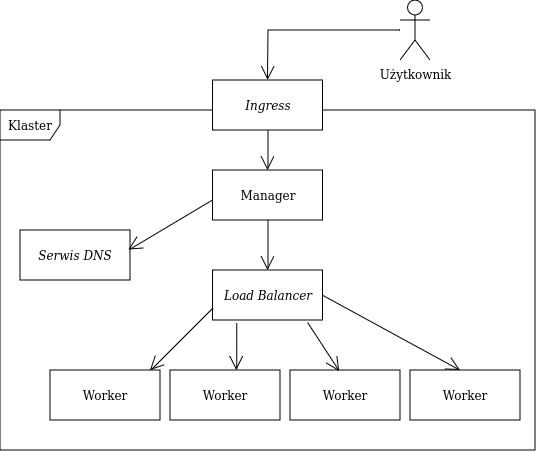
\includegraphics{img/4/k8s.png}
		}
		\caption[Diagram prototypu klastra Kubernetes]{Diagram przedstawiający elementy prototypu klastra Kubernetes wdrożonego dla systemu STOS. Źródło własne.}
		\label{diagramk8s}
	\end{center}
\end{figure}

W ramach projektu inżynierskiego powstał prototyp takiego klastra, zawierający symulowaną architekturę systemu STOS (\ref{diagramk8s}). Umożliwiał on dynamiczne skalowanie ilości instancji serwisu kompilującego \textit{(worker)}, odpowiedzialnego za ewaluację zadań przesyłanych przez studentów, jak i~monitorowanie stanu wszystkich działających w~ramach systemu usług.

Oprócz samych komponentów systemowych STOSu zaprojektowany klaster oferował również szereg usług dodatkowych. Jedną z nich jest wbudowany serwer DNS, który znacząco ułatwia konfigurację komunikacji pomiędzy usługami systemu\cite{k8sDns}. Drugim najważniejszym komponentem był „service” w~kontekście Kubernetesa, pełniący funkcję load-balancera dla poszczególnych serwisów kompilujących \textit{(worker)}. Tym sposobem, zagwarantowano równomierne obciążenie każdej instancji serwisu, bez względu na ilość działających kontenerów\cite{k8sService}. Ostatnim z elementów klastra była usługa Ingress, pozwalająca na jednoznaczne zdefiniowane punktu dostępu do serwisów klastra ze środowiska zewnętrznego, którym w~tym prototypie był serwis zarządzający \textit{(manager)}\cite{k8sIngress}.

\subsection{Koncepcja wdrożenia a~dynamika wymagań}
Jednakże, w~trakcie prac i~w~kontekście dynamicznie zmieniających się wymagań, wdrożenie systemu STOS jako klaster oparty na orkiestratorze kontenerów okazało się przedsięwzięciem bardziej skomplikowanym, niż mogłoby się to wydawać na początku prac. Wymaganiem była możliwość kontrolowania kontenerów Docker z poziomu samej aplikacji, będącej częścią STOS-u. Łączyło się ono z większym stopniem złożoności rozwiązania spowodowanej wprowadzeniem dodatkowych komponentów lub zastosowaniem zaawansowanych wzorców projektowych przeznaczonych dla skonteneryzowanych aplikacji rozproszonych, takich jak „wózek boczny” \textit{(sidecar pattern)}\cite{k8sPatterns}. Projekt rozwiązania opierającego się na klastrze Kubernetes i~korzystający z dodatkowych komponentów systemowych przedstawiono na rysunku \ref{diagramk8sFinal}.

\begin{figure}[!h]
	\begin{center}
		\resizebox{0.7\textwidth}{!} {
			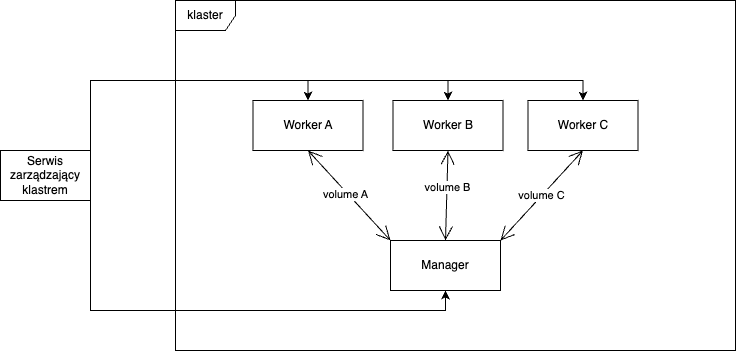
\includegraphics{img/4/k8sFinal.png}
		}
		\caption[Diagram prototypu klastra Kubernetes po zmianie architektury]{Diagram przedstawiający ogólną architekturę systemu wdrożonego na klaster Kubernetes po zmianie wymagań dotyczących konteneryzacji serwisu kompilującego \textit{(worker)}. Źródło własne.}
		\label{diagramk8sFinal}
	\end{center}
\end{figure}

Zgodnie z wymaganiami, których źródłem są istniejące komponenty systemu STOS, komunikacja między kontenerem kompilującym i~serwisem zarządzającym \textit{(manager)} musi być zrealizowana za pomocą współdzielonych katalogów. Taki mechanizm oferowany jest zarówno w~postaci wolumenów w~Dockerze\cite{dockerVolume}, jak i~StatefulSet w~Kubernetes\cite{k8sStateful}. Za zlecanie ewaluacji zadania i~dynamiczne uruchamianie serwisu kompilującego \textit{(worker)}, w~tym modelu systemu odpowiedzialny jest dedykowany serwis uruchomiony poza klastrem, posiadający pełny dostęp do mechanizmów zarządzania tym klastrem.

Dodanie serwisu, którego awaria wiąże się z awarią całego systemu w~postaci zewnętrznego serwisu nadzorującego stan klastra i~cykl życia kontenerów to tylko część wad tego rozwiązania. Przy zastosowaniu kontenerów, które muszą utrzymywać swój stan, czyli skorzystaniu z technologii StatefulSet, dodatkowym czynnikiem przyczyniającym się do skomplikowania aplikacji jest zarządzanie współdzielonymi wolumenami, z których korzysta serwis zarządzający \textit{(manager)} w~celu komunikacji z instancjami serwisu kompilującego \textit{(worker)}. Dodatkowo niemożliwe staje się zastosowanie wbudowanego w~klaster Kubernetes serwisu odgrywającego rolę serwisu odpowiadającego za sprawiedliwy rozkład żądań przychodzących do poszczególnych instancji serwisów \textit{(load-balancer)}, co wiąże się z koniecznością ręcznej implementacji tej funkcjonalności.

Z racji rosnącego stopnia skomplikowania wdrożenia systemu STOS za pomocą klastra Kubernetes, podjęta została decyzja o~zaprojektowaniu rozwiązania nieopierającego się na technologii orkiestracji kontenerów.


% --------------
% Konteneryzacja i alternatywy
% -------------

% LTex: language=pl

\section{Konteneryzacja i~rozwiązania alternatywne}
\subsection{Wirtualizacja}
Pojęcie wirtualizacji zaczęło pojawiać się w~użyciu już w~latach siedemdziesiątych XX wieku. W~1974 opublikowany został artykuł autorstwa Geralda J. Popka i~Roberta P. Goldberga, którego autorzy wprowadzili sformalizowaną definicję wirtualizacji. Główne założenia proponowanej definicji opierały się na twierdzeniu o~zachowaniu relacji równoważności pomiędzy pojedynczymi instrukcjami i~sekwencjami instrukcji wykonywanymi na maszynie fizycznej i~maszynie wirtualnej\cite{virtualization}.

\begin{lemat}
	Niech $i$ oznacza dowolną instrukcję, $S$ oznacza stan maszyny fizycznej, natomiast $S'$ stan maszyny wirtualnej, w~taki sposób, że $S' = f(S)$. Wykonanie instrukcji na obu maszynach wiąże się z identyczną interpretacją takiej instrukcji w~obu środowiskach, tak że $i(S) = i(S')$.
\end{lemat}

\begin{lemat}
	Ponieważ wszystkie pojedyncze instrukcje $i$ interpretowane są w~ten sam sposób na maszynie fizycznej o~stanie $S$ i~maszynie wirtualnej o~stanie $S'$, wszystkie skończone zbiory uporządkowane instrukcji $t = (i_1, i_2, \ldots, i_n)$ również interpretowane są w~ten sam sposób dla obu środowisk, tak że $f(t(S)) = f(t(S'))$.
\end{lemat}

\noindent Oprócz formalnych dowodów dotyczących zachowania maszyny i~właściwości, jakie powinna wykazywać, artykuł ten wprowadził pojęcie „monitora maszyny wirtualnej” - programu zarządzającego zachowaniem i~zasobami wirtualizowanej maszyny i~wskazał również główne moduły składające się na taki program. Na przestrzeni lat pojęcie to przekształciło się w~„nadzorcę” \textit{(hypervisor)}, wraz z podziałem na 2 główne typy programu-nadzorcy -- nadzorca typu pierwszego \textit{(type 1 hypervisor)} i~nadzorca typu drugiego \textit{(type 2 hypervisor)}.

\noindent O~wiele młodszą technologią jest z kolei konteneryzacja, która, mimo podobieństwa do wirtualizacji, nie spełnia wszystkich wymogów formalnych prezentowanych powyżej, w~szczególności tych, dotyczących zachowania relacji równoważności pomiędzy pojedynczymi instrukcjami procesora i~powiązania wyłącznie z architekturą fizyczną maszyny. Mimo tego jest ona szeroko wykorzystywana w~rozwiązaniach o~szerokim spektrum skali -- od projektów hobbystycznych do rozwiązań klasy przemysłowej.

\subsection{Kontenery a~maszyny wirtualne}
W celu przedstawienia głównych różnic pomiędzy wirtualizacją i~konteneryzacją należy przeanalizować architekturę rozwiązań implementujących te technologie -- silnik konteneryzacji, nadzorcę typu pierwszego \textit{(type 1 hypervisor)} i~nadzorcę typu drugiego \textit{(type 2 hypervisor)} (rysunek \ref{diagramWirtualizacja}).

\begin{figure}[!h]
	\begin{center}
		\resizebox{0.7\textwidth}{!} {
			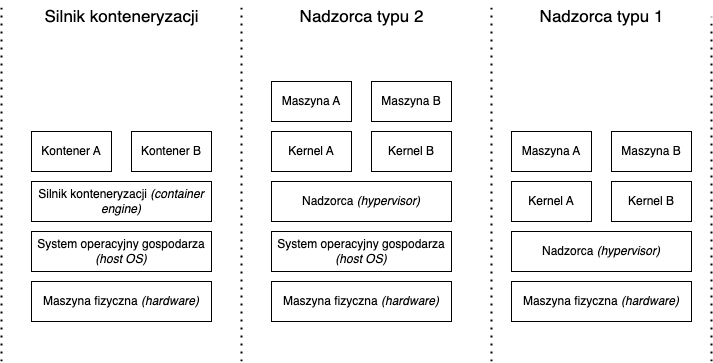
\includegraphics{img/4/wirtualizacja.png}
		}
		\caption[Porównanie silnika konteneryzacji i~programów-nadzorców]{Schemat przedstawiający i~porównujący architekturę silnika konteneryzacji i~programów-nadzorców maszyn wirtualnych. Źródło własne.}
		\label{diagramWirtualizacja}
	\end{center}
\end{figure}

\subsubsection{Nadzorca typu pierwszego \textit{(type 1 hypervisor)}}
Programy nadzorcy typu pierwszego najczęściej wykorzystywane są w~rozwiązaniach przemysłowych, wymagających zaawansowanych rozwiązań z zakresu monitorowania nadzorowanych maszyn wirtualnych i~wydajności przetwarzania. Do najpopularniejszych ogólnodostępnych programów zaliczających się do tej rodziny należą, między innymi, Proxmox, xcp-ng i~KVM. Nadzorca typu pierwszego pełni rolę systemu operacyjnego zainstalowanego na maszynie fizycznej i~posiada bezpośrednią kontrolę nad jej zasobami sprzętowymi. Dzięki temu wirtualizacja realizowana przy pomocy oprogramowania tego typu charakteryzuje się blisko natywną wydajnością wirtualizowanych maszyn. Każda maszyna wirtualna stanowi w~pełni oddzielną maszynę logiczną, z wydzielonym jądrem systemu operacyjnego i~dedykowaną ilością zasobów fizycznych, takich jak pamięć operacyjna czy rdzenie lub wątki procesora. Ponadto, z racji ich powszechnego wykorzystania w~rozwiązaniach klasy przemysłowej, bardzo często programy-nadzorcy typu pierwszego posiadają wbudowane funkcjonalności zarządzania systemami (klastrami) składającymi się z wielu maszyn fizycznych podobne do rozwiązań obecnych w~systemach orkiestracji kontenerów, takich jak Kubernetes.

\subsubsection{Nadzorca typu drugiego \textit{(type 2 hypervisor)}}
Nadzorca typu drugiego to najbardziej rozpowszechniony program oferujący pełną wirtualizację. Reprezentantami tej rodziny programów-nadzorców maszyn wirtualnych są programy Oracle VirtualBox, Parallels i~VMware. Nadzorca typu drugiego to program uruchamiany na dowolnej maszynie z uprzednio zainstalowanym systemem operacyjnym, co czyni go najbardziej przyjaznym rozwiązaniem do celów konsumenckich lub prototypowania. Mimo instalacji na istniejącym systemie nadzorca typu drugiego oferuje te same funkcjonalności związane z wirtualizacją co nadzorca typu pierwszego, alokując dedykowane zasoby dla poszczególnych maszyn wirtualnych, którymi zarządza, w~tym osobny kernel (jądro) systemu dla każdej maszyny logicznej. Wygoda użytkowania niesie za sobą jednak koszty związane z wydajnością maszyn, ponieważ system operacyjny, na którym uruchomiony jest program-nadzorca wnosi znaczące opóźnienia związane z komunikacją systemu w~maszynie wirtualnej z zasobami sprzętowymi kontrolowanymi przez system operacyjny gospodarza. Ponadto, funkcjonalności takie jak zarządzanie systemami składającymi się z wielu maszyn fizycznych nie są wbudowane w~programy zaliczające się do tej rodziny, zamiast tego nacisk kładziony jest na łatwość użytkowania aplikacji przez użytkownika końcowego.

\subsubsection{Silnik konteneryzacji}
Konteneryzacja to technologia, pozwalająca na uzyskanie większości funkcjonalności wirtualizacji wykorzystując stosunkowe małe maszyny logiczne nazywane „kontenerami”. Główna różnica pomiędzy wirtualizacją i~konteneryzacją polega na wykorzystaniu systemu operacyjnego gospodarza. O~ile w~przypadku wirtualizacji, z wykorzystaniem nadzorcy typu pierwszego i~drugiego, każda maszyna wirtualna posiada swój własny kernel (jądro) systemu operacyjnego, w~przypadku konteneryzacji system operacyjny, w~szczególności jego jądro, jest współdzielone między wszystkie kontenery. Skutkuje to zmniejszeniem rozmiaru kontenerów, które nie muszą zawierać w~sobie obrazu całego systemu i~szybszym czasem uruchamiania, które są często głównymi czynnikami przemawiającymi za zastosowaniem kontenerów nad maszynami wirtualnymi. Jednakże, z racji ścisłego powiązania z systemem gospodarza, na którym działa kontener, lemat dotyczący zachowania relacji równoważności instrukcji dotyczący maszyny wirtualnej Popka i~Goldberga\cite{virtualization} nie jest zachowany dla każdego kontenera uruchomionego na tej samej architekturze. Przykładowo, kontener oparty na systemie Linux może zostać uruchomiony na maszynach gospodarza o~różnych wersjach kernela (jądra) systemu, rezultatem czego może być różna interpretacja wywołań systemowych dla identycznych wywołań w~każdym z tych kontenerów. Dlatego, w~świetle tego artykułu, konteneryzacja nie jest stricte rodzajem wirtualizacji. Z praktycznego punktu widzenia, oznacza to niemożność wykorzystania kontenerów opartych na pewnym systemie operacyjnym $O_a$ na maszynie o~systemie operacyjnym $O_b$, gdzie kernele (jądra) systemów $O_a$ i~$O_b$ są ze sobą niekompatybilne -- przykładem takiej sytuacji jest próba uruchomienia kontenera korzystającego z systemu Microsoft Windows ($O_a$) na maszynie opartej na systemie Linux ($O_b$).

\subsection{Wirtualizacja a~platforma serwerowa dla systemu STOS-new}
Z racji wystąpienia komplikacji, o~których była mowa w~poprzednim podrozdziale, w~ramach poszukiwania rozwiązania alternatywnego dla konteneryzacji, naturalnym wyborem była analiza wirtualizacji jako technologii stanowiącej podstawę wdrożenia systemu. Pierwszą decyzją, którą należało podjąć, był wybór typu nadzorcy \textit{(hypervisor)} i~konkretnej implementacji tego rozwiązania. W~świetle doświadczeń z systemami orkiestracji kontenerów naturalnym wyborem był system oparty na nadzorcy typu pierwszego \textit{(type 1 hypervisor)}; wiele z implementacji tego właśnie typu nadzorcy oferuje funkcjonalności z zakresu zarządzania wieloma maszynami fizycznymi, co było jednym z wymagań dla wdrożonego systemu. Dwiema implementacjami takiego systemu, których zastosowanie było rozważane, były Proxmox i~xcp-ng\cite{proxmox, xcp}. Oba z tych rozwiązań oferują bardzo podobne rozwiązania, lecz ostatecznie wybrano xcp-ng jako system nadzorcy, na podstawie którego realizowana jest wirtualizacja serwisów w~ramach platformy serwerowej dla systemu STOS-new.


% LTex: language=pl
\chapter{Propozycje rozwoju aplikacji}

% LTex: language=pl
\section{Dedykowane kontenery do kompilacji lub interpretacji większej ilości języków programowania (autor: Adam Niesiobędzki)}
Obecny system wykorzystywany jest głównie na zajęciach laboratoryjnych i~projektowych z~przedmiotów Podstawy Programowania oraz Algorytmy i~Struktury Danych, na których programowanie odbywa się z~wykorzystaniem języka programowania C++. Jego funkcjonalność mogłaby zostać rozszerzona poprzez implementację dedykowanych kontenerów przeznaczonych do kompilacji lub interpretacji większej ilości języków programowania, takich jak Python, C\# lub Java. Kod źródłowy rozwiązania byłby przekazywany do odpowiedniego kontenera odpowiedzialnego za kompilację lub interpretację na podstawie danych zadania pozyskanych z~zewnętrznego systemu STOS-WEB, utworzony plik wykonywalny byłby następnie przetwarzany i~oceniany w taki sam sposób jak dzieje się to obecnie. Pozwoliłoby to na większą dowolność w wyborze technologii wykorzystanej do implementacji rozwiązania oraz wdrożenie systemu w proces kształcenia i~automatyzacji oceniania na zajęciach laboratoryjnych i~projektowych z~większej ilości przedmiotów. Kursy cechujące się oczekiwanym rezultatem wykonanego zadania w~obecnym toku nauczania kierunku Informatyka na Politechnice Gdańskiej, które mogłyby wykorzystać rozbudowany system to na przykład Programowanie Obiektowe, Metody Numeryczne, Platformy Technologiczne oraz Sztuczna Inteligencja.

% LTex: language=pl
\section{Serwis DNS (autor: Tymoteusz Paliński)}
Z racji na dość wysoki stopień skomplikowania architektury wdrożenia, w aktualnej fazie projektu dodawanie kolejnych maszyn i~usług zostało uznane za niewskazane -- zarówno przez ramy czasowe projektu, jak i~potencjalnie wysoki próg wejścia dla obecnego i~przyszłych administratorów systemu STOS. Nie oznacza to jednak, że architektura wdrożenia nie oferuje przestrzeni na dodanie komponentów usprawniających działanie i~zwiększających niezawodność platformy serwerowej dla systemu STOS.
\newline \noindent Jednym z~takich serwisów jest lokalny serwer DNS działający w~ramach klastra xcp-ng. W~aktualnej
implementacji platformy serwerowej komunikacja pomiędzy poszczególnymi maszynami odbywa się za pomocą bezpośredniej adresacji poprzez adresy IP każdej z maszyn. Podejście to cechuje się wysoką wrażliwością na zmiany konfiguracji sieciowej rozwiązania i~może skutkować wystąpieniem trudnych do wykrycia błędów podczas przyszłego rozwoju aplikacji. Dodanie własnego lokalnego serwera DNS pozwoliłoby na zniwelowanie tego problemu, jak i~potencjalne wprowadzenie dodatkowych mechanizmów zwiększających bezpieczeństwo systemu, takie jak wprowadzenie listy niedostępnych domen lub skorzystanie z mechanizmu \textit{round robin} w celu zwiększenia przepustowości ruchu sieciowego\cite{roundRobin}.
\newline \noindent Do wdrożenia takiego rozwiązania można wykorzystać gotowe oprogramowanie otwartoźródłowe, takie jak \textit{Pi-Hole} lub \textit{Unbound}\cite{pihole, unboundDns}. Obie z tych aplikacji oferują funkcjonalności lokalnego serwera DNS, aczkolwiek \textit{Unbound} charakteryzuje się większym stopniem optymalizacji w kontekście bezpieczeństwa sieci i~mechanizmu pamięci podręcznej zewnętrznych dla rekordów pochodzących z~serwerów zewnętrznych; z kolei \textit{Pi-Hole} cechuje się prostszą konfiguracją, lecz zazwyczaj używany jest w sieciach domowych jako prosty serwis \textit{cache} dla zewnętrznych serwerów DNS i wykorzystywany jest jako usługa \textit{AdBlock} blokująca reklamy w sieciach domowych. Zważając na ilość rozwiązań przemysłowych wykorzystanych w ramach architektury wdrożenia, serwis \textit{Unbound} wydaje się naturalnym wyborem dla wdrożenia go jako lokalnego serwera DNS w ramach klastra maszyn wirtualnych.



% LTex: language=pl
\section{Kontener wykonujący oraz oceniający}


% LTex: language=pl
\section{Gromadzenie metryk i ich wizualizacja}
W celu rozszerzenia możliwości monitorowania stanu systemu za pomocą istniejącej implementacji platformy Elasticstack proponujemy użycie serwisu Metricbeat opracowany przez firmę Elastic, który jest spedytorem metryk generowanych przez określoną usługę. Serwis oferuje szereg zintegrowanych narzędzi, umożliwiających na gromadzenie danych z kolejek, usług chmurowych, baz danych i systemów operacyjnych \cite{metricbeat}. Jego działanie polega na okresowym odpytywaniu monitorowanych serwisów, poprzez wywoływanie komend lub żądań HTTP. W przypadku braku odpowiedzi po zdefiniowanym czasie Metricbeat przesyła zdarzenie zawierające błąd w celu uproszczenia diagnostyki \cite{metricbeat_work}. Jego konfiguracja jest analogiczna do istniejącego serwisu Filebeat i opiera się na uruchomieniu modułu jako usługa na systemie linuksowym z konfiguracją zdefiniowaną w pliku \textit{metricbeat.yml}.


% LTex: language=pl
\section{Modyfikacja serwisu STOS (autor: Łukasz Nowakowski)}
By zwiększyć elastyczność systemu, proponujemy zmodyfikowanie obecnego interfejsu systemu STOS. Obecna implementacja funkcji komunikacji z serwisem polega na porównaniu wartości otrzymanego nagłówka żądania do zdefiniowanego zestawu obsługiwanych komend i~jego obsłudze. W~przypadku potrzeby rozwoju należy rozwinąć instrukcję warunkową i~dodać do niej obsługę nowego parametru oraz ustawić ten nagłówek w~miejscu wysyłania żądania. Zmniejsza to czytelność i~zwiększa trudność w~utrzymaniu kodu. Ze względu na umieszczenie obsługi w~bloku \textit{try-catch}, nie istnieje dedykowana obsługa błędu, co utrudnia diagnostykę w~przypadku jego wystąpienia. Proponujemy stworzenie nowego interfejsu komunikacyjnego obsługującego żądania HTTP posiadającego trzy punkty końcowe:
\begin{itemize}
    \item Otrzymywanie metadanych zadania z kolejki -- punkt końcowy znajdujący się pod adresem \textit{/tasks}, wywoływany żądaniem typu \textit{GET}. Ma za zadanie zwrócić metadane zadania z kolejki i~je usunąć. Zwracane dane będą zawierać identyfikatory plików testów, plików przesłanych przez studenta oraz zadania, które jest rozwiązywane. Usuwanie zadań z kolejki powinno być synchronizowane.
    \item Otrzymywanie pliku o~określonym identyfikatorze -- punkt końcowy znajdujący się pod adresem \textit{/files/<id:int>}, wywoływany żądaniem typu GET. Zwraca plik oraz jego typ. Rozdział na możliwość pobierania pojedynczych pilików zamiast całego zestawu, pozwana na zastosowanie systemu pamięci podręcznej, która pozwoli na pominięcie kroku pobierania kilkukrotnie tego samego zbioru plików, szczególnie plików zawierających zadanie oraz testy, które w~większości przypadków pozostają niezmienione.
    \item Zapisywanie wyniku zadania -- punkt końcowy znajdujący się pod adresem \textit{/tasks/<id:int>}, wywoływany żądaniem typu POST. Zapisuje wynik dla każdego z testów dla danego studenta, dla zadania określanego w~żądaniu.
\end{itemize}

Każdy z punktów końcowych powinien być obsłużony w~osobnej funkcji i~posiadać odpowiednią obsługę wyjątków. Do implementacji sugerujemy użycie technologii PHP, Python, Java lub C\# oraz opcjonalnie frameworków Laravel, Django, Flask, Spring lub ASP.NET. Sugerowane działanie zostało przedstawione na schemacie \ref{stos-suggestion}.
\begin{figure}[!h]
	\begin{center}
		\resizebox{1.0\textwidth}{!} {
			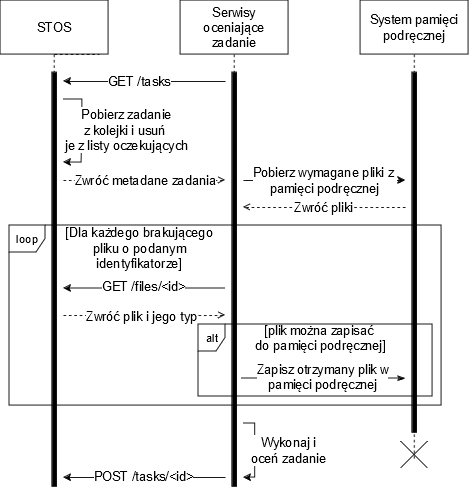
\includegraphics{img/5/stos-suggestion.png}
		}
		\caption[Schemat działania zaproponowanego serwisu. Źródło własne.]{Schemat działania zaproponowanego serwisu. Źródło własne.}
    \label{stos-suggestion}
	\end{center}
\end{figure}


% LTex: language=pl
\section{Komunikacja przez kolejki (autor: Adam Niesiobędzki)}
System kolejkowy jest fragmentem oprogramowania umożliwiającym komunikację między serwisami aplikacji niezależnie od języka programowania, w~którym są napisane. W~systemie kolejkowym producentem określa się komponent tworzący dane, a~konsumentem komponent, który dane odbiera. Możliwe jest, że komponent jest jednocześnie zarówno producentem, jak i~konsumentem. Kolejka przechowuje wiadomości lub dane wysłane przez producenta, dopóki nie zostaną pobrane i~przeprocesowane przez konsumenta. Pozwala to na separację aplikacji od siebie, tak, aby każda część systemu mogła wykonywać swoją pracę niezależnie od pozostałych. Podstawową zaletą systemu kolejek nad REST API jest gwarancja, że nadana wiadomość nie zostanie stracona w~wyniku dysfunkcji konsumenta. W~tworzonym systemie komunikacja za pośrednictwem systemu kolejkowego mogłaby występować między zewnętrznym systemem STOS a~systemem oceniającym rozwiązania zadań, gdzie zewnętrzny system STOS umieszczałby nowo dodane zadania do kolejki, które następnie byłyby z niej pobierane przez instancje systemów oceniających. Dzięki zastosowaniu takiego kanału komunikacji zamiast obecnych żądań HTTP nie byłoby konieczności ciągłego odpytywania API o~pojawienie się nowych zadań, komponenty systemu byłyby ze sobą mniej powiązane, a~skalowanie systemu mogłoby się odbywać nie tylko poprzez zrównoleglenie kompilacji i~oceny zadań wewnątrz kontenerów, ale także poprzez utworzenie licznych instancji systemów sprawdzających zadania pracujących na różnych maszynach fizycznych, gdzie każda z instancji pozyskiwałaby zadania z ogólnodostępnej kolejki oraz umieszczałaby rozwiązania w~drugiej, której konsumentem jest STOS. Dodatkową zaletą systemu kolejkowego jest możliwość przechowywania komunikatów po ich odczytaniu, co pozwala na powtórzenie przetwarzania komunikatu nawet w~przypadku awarii maszyny, która pobrała z niej wiadomość, co zwiększyłoby niezawodność systemu. Argumentem przemawiającym przeciw wprowadzeniu systemu kolejkowego jest fakt, że byłoby to kolejne narzędzie w~zestawie technologii wchodzących w~skład systemu, zwiększając jego skomplikowanie. Dodatkowo potencjalna dysfunkcja tego kanału komunikacji stanowiłaby zagrożenie dla działania całego systemu, jednak systemy kolejkowe takie jak Apache Kafka lub RabbitMQ, to systemy stosowane w~licznych rozwiązaniach klasy przemysłowej, są niezawodne i~dobrze przetestowane.
\begin{figure}[!ht]
	\begin{center}
		\resizebox{1.0\textwidth}{!} {
			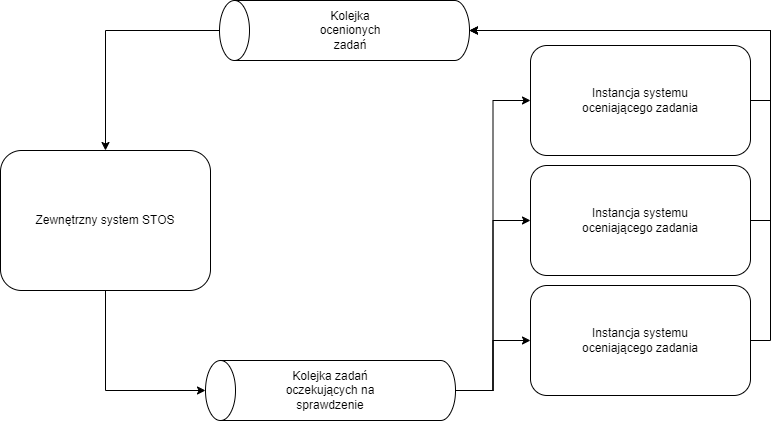
\includegraphics{img/5/system-kolejkowy.png}
		}
		\caption[Schemat komunikacji opartej na systemie kolejkowym. Źródło własne.]{Schemat komunikacji opartej na systemie kolejkowym. Źródło własne.}
    \label{stos-queue}
	\end{center}
\end{figure}

% LTex: language=pl
\chapter{Podsumowanie (autor: Łukasz Nowakowski)}

Istniejący system został przeanalizowany i opisany w tej pracy, zarówno pod względem uruchamiania jak i przepływu sterowania. Zostały przebadane możliwości użycia istniejących komponentów i ich skalowania. Moduł kompilujący oraz serwis STOS zostały zintegrowane z obecnym rozwiązaniem. Moduł kompilujący wymaga osobnego zestawu katalogów, w celu uniknięcia konfliktów między działającymi równolegle wieloma instancjami rywalizującymi o dane z nazwanego potoku, co zostało rozwiązane w docelowym systemie. 
\newline \indent W celu zwiększenia niezawodności systemu, uruchomione kontenery są zarządzane przez naszą aplikację, która zapewnia stałą ilość działających kontenerów i ich wznawianie w przypadku awarii, aż do ilości na którą pozwalają dostępne zasoby obliczeniowe. Decyzja o użyciu takiego rozwiązania zamiast komercyjnych platform konteneryzacji, takich jak Kubernetes albo Docker Swarm, wiązała się z założeniem działania zagnieżdżonego kontenera z modułem kompilującym. Logi generowane przez aplikację są przesyłane do platformy Elasticstack, będąca centralnym punktem gromadzącym i wizualizującym logi. Jako mechanizm sprawiedliwej oceny uniezależniony od obecnej ilości dostępnych zasobów obliczeniowych, sugerowane jest zliczanie niskopoziomowych operacji. Mechanizm ten nie został zaimplementowany, ze względu na skompilowanie i priorytet pozostałych aspektów.
\newline \indent Utworzony system jest przystosowany do obsługi plików pobieranych z serwisu STOS oraz do ich kompilacji. Aplikacja została przetestowana poprzez testy jednostkowe, testy manualne oraz uruchomioną, kilkudniową symulację. W celu zapewnienia jakości kodu, zostało zintegrowane narzędzie Prospector, które służy do statycznej analizy kodu. By umożliwić prosty rozwój oprogramowania, rozwiązanie zostało oparte na udokumentowanych interfejsach, które zawierają gotowe implementacje. Dla modułów których funkcjonalności ze względów na brak plików źródłowych nie udało się odtworzyć, zostały utworzone symulacje, które w dalszych etapach rozwoju powinny zostać podmienione.
\newline \indent Rozwiązanie zostało umieszczone na serwerze politechniki. W tym celu, zostały utworzone maszyny wirtualne na środowisko produkcyjne oraz deweloperskie, serwer logów oraz maszynę z narzędziem Xen Orchestra UI. Zastosowanie maszyn wirtualnych nadzorcy pierwszego stopnia xcp-ng które jest sprawdzonym, komercyjnym rozwiązaniem, umożliwia na proste zarządzanie i monitorowanie maszyn wirtualnych.
\newline \indent Obsługa systemu została zawarta spisana w plikach Markdown. Prezentują one sposoby konfiguracji i rozwoju systemu. Uruchamianie systemu zostało sprowadzone do uruchomienia pojedynczego skryptu.
\newline \indent Utworzony system spełnia większość określonych na początku założeń. Ze względu na późny termin otrzymania kodu źródłowego oraz braki pojedynczych plików, nie wszystkie funkcjonalności mogły zostać zaimplementowane. Do atutów rozwiązania możemy zaliczyć prostotę analizy działania i rozwoju, skalowalność oraz użycie nowoczesnych narzędzi. System po zaimplementowaniu brakujących modułów może stanowić udoskonaloną alternatywę dla platformy STOS, gotową do użycia w warunkach produkcyjnych.



% Bibliografia
\printbibliography

% Autorstwo
\newpage
\thispagestyle{empty}
\noindent Zakres odpowiedzialności członków zespołu:
\newline Tymoteusz Paliński:
\newline Wdrożenie rozwiązania na serwer, konfiguracja i przygotowanie maszyn wirtualnych, opracowanie prototypu wdrożenia na klastrze Kubernetes, opracowanie architektury rozwiązania.
\newline Adam Niesiobędzki: 
\newline Implementacja rozwiązania, integracja komponentów, opracowanie architektury rozwiązania, implementacja kontenera kompilującego i uruchamiającego zadania opartego na Wine, opracowanie prototypu systemu logowania opartego na Graylog.
\newline Łukasz Nowakowski:
\newline Analiza systemu, opracowanie architektury rozwiązania, implementacja symulatorów serwisów STOS oraz Evaluator, przygotowanie instrukcji do serwisu Elasticstack, implementacja komponentu logowania.
\newpage
\end{document}
